% Created 2019-05-15 Wed 12:52
% Intended LaTeX compiler: pdflatex
\documentclass[english,zadani,odsaz]{fitthesis}
\renewcommand\title[1]{}
%%% Local Variables:
%%% mode: latex
%%% TeX-master: "projekt.org"
%%% End:

\projectinfo{
  project={BP},
  year={2019},
  date=\today,
  title.cs={Název práce},
  title.en={Thesis title},
  %title.length={14.5cm},
  author.name={Jakub},
  author.surname={Zárybnický},
  department={UITS},
  faculty={FIT},
  supervisor.name={Ondřej},
  supervisor.surname={Lengál},
  supervisor.title.p={Ing.},
  supervisor.title.a={Ph.D.},
  keywords.cs={Sem budou zapsána jednotlivá klíčová slova v českém (slovenském) jazyce, oddělená čárkami.},
  keywords.en={Sem budou zapsána jednotlivá klíčová slova v anglickém jazyce, oddělená čárkami.},
  abstract.cs={Do tohoto odstavce bude zapsán výtah (abstrakt) práce v českém (slovenském) jazyce.},
  abstract.en={Do tohoto odstavce bude zapsán výtah (abstrakt) práce v anglickém jazyce.},
  declaration={Hereby I declare that this bachelor's thesis was prepared as an
    original author’s work under the supervision of Ing. Ondřej Lengál,
    Ph.D. All the relevant information sources used during preparation of this
    thesis are properly cited and included in the list of references.},
  %acknowledgment={Here it is possible to express thanks to the supervisor and
  %  to the people which provided professional help (external submitter, consultant, etc.).},
  extendedabstract={Do tohoto odstavce bude zapsán rozšířený abstrakt práce v
    českém jazyce, bude mít rozsah 2 až 6 normostran a bude obsahovat úvod,
    popis vlastního řešení a shrnutí a zhodnocení dosažených výsledků.},
}

\usepackage{minted}
\usepackage[figure,table,listing]{totalcount}
\date{\today}
\title{}
\hypersetup{
 pdfauthor={},
 pdftitle={},
 pdfkeywords={},
 pdfsubject={},
 pdfcreator={Emacs 26.1 (Org mode 9.1.9)}, 
 pdflang={English}}
\begin{document}

% * (front matter)                                              :ignoreheading:
\maketitle
\setlength{\parskip}{0pt}
{\hypersetup{hidelinks}\tableofcontents}
\iftotalfigures\listoffigures\fi
\iftotaltables\listoftables\fi
\iftotallistings\listoflistings\fi
\iftwoside\cleardoublepage\fi
\setlength{\parskip}{0.5\bigskipamount}

\chapter{Introduction}
\label{sec:orgbe06a57}
Imagine you are building an application for an event your company is
organizing. There will not be reliable internet connection in the area of the
event, so it needs to work offline. You are on a tight budget, so implementing
one version for each platform is not feasible, but it needs to work reliably
across all mobile platforms and ideally in the browser as well. What is the
easiest way to accomplish that?

This situation is exactly where a rather new concept of a Progressive Web
Application (PWA) is the best solution. Generally said, a PWA is website
capable of running offline, using mobile notifications, or synchronizing data in
the background, things previously specific to native mobile applications.

Moreover, consider that the application server is written in Haskell, a
statically typed, purely functional programming language. We want to reuse the
business logic already written there to avoid duplicating code, so we search for
a way to write a Web application in Haskell. We find many resources and a
quickly growing community but while creating the application, we soon step into
the unknown. A medium-scale application needs a large number of capabilities,
but the ecosystem of frontend Haskell is not yet big enough to support many of
them, and many libraries in the area are either exploratory or one-off projects.
In this work, we will try to fill in many such gaps, with the goal of creating a
framework for creating Progressive Web Applications in Haskell.

We will first go through the details of what a Progressive Web Application is
(Chapter~2) and what features are common in today's Web frameworks (Chapter 3),
followed by a quick introduction to Haskell and an evaluation of the Haskell
ecosystem in the area of Web development (Chapter 4). After seeing what is
missing, we will walk through the implementation of several libraries in the
area (Chapter 5), have a look at how to create an application using these
components (Chapter 6), and conclude with four separate case studies (Chapter
7).

The source code for this work is available online
\url{https://github.com/zarybnicky/thesis}, and also at \url{https://tapaw.dev}, where the
live versions of the applications created here are also available.

\chapter{What is a PWA?}
\label{sec:org0b3f122}
\section{Web development trends}
\label{sec:orgeba9d43}
Today, web pages are more than just static HTML markup. We have moved from the
Web without JavaScript where any interactions needed to be processed by the
server, through using JavaScript just for animations and small ease-of-use
features, to building entire applications in JavaScript that only talk to
servers in the background.

When JavaScript received the ability to execute HTTP requests and get or save
data in the background, a technology then called AJAX, it was only used for
small pieces of functionality. Only later came the concept of Single Page
Applications (SPA), where the application was only loaded once at the beginning
and only communicated in JSON or XML afterwards. This brought new challenges to
JavaScript developers, challenges like rendering templates in the browser,
managing application state or routing (the mapping between application state and
the URL displayed in the address bar of a browser).

Not only was the Web developing, but also mobile devices and their applications,
also called native applications today (as opposed to web applications). These
applications had access to the full capabilities of the devices they were
running on and could, at the start, do a lot more than a web application.

This meant that a company that wanted to reach as many users as possible had to
develop many versions of the same application: for the web, desktop, and also
for several varieties of mobile devices. Later came projects like Cordova
and Electron that made it possible to use JavaScript and other web technologies
not only in the browser but also in native mobile and desktop applications, but
the ambition of making the web the universal application platform stayed there.

Under the umbrella of the Web Platform project, many new JavaScript extensions
were developed, interfaces that gave JavaScript access to many facets of the
device on which the browser runs. Some examples are the Location API that gives
access to the GPS location of a device, or the Screen Capture API that enables a
website to capture the screen of the browser or another application.

Given that the device type most often for browsing the Web is a mobile device
and has been for a few years already \cite{mobile-stats}, the effort to equalize
the capabilities of web and mobile applications is still ongoing, and a large
step towards this goal is the concept of a Progressive Web Application.

\section{Progressive Web Applications}
\label{sec:org42be0c2}
The term Progressive Web Application (PWA) is an umbrella term for several
relatively new, closely related technologies. While many of them are useful on
all devices, the main target audience are mobile Web browsers.

The goal of the PWA project is to enable developers to create Web applications
that are equal in functionality to native ones in many domains like shopping or
productivity. The technologies that comprise the term PWA allow applications to
be installable directly from a web browser to the device, to become capable of
working offline, to use some background services of the device, all features
formerly only available to mobile applications. To use the marketing terms,
converting a web application into a PWA improves user experience and brings
higher user engagement and retention.

The term PWA has an exact specification in a checklist created by Google
\cite{pwa_checklist}, which describes two levels of PWAs, a Baseline PWA and an
Exemplary PWA. The defining characteristics of a Baseline PWA are, as quoted
directly from the checklist:

\begin{itemize}
\item Pages are responsive on tablets and mobile devices.
\item All application URLs load while offline.
\item Site uses cache-first networking.
\item Page transitions do not feel like they block on the network.
\item Pages use the History API.
\item Each page has a URL.
\item Metadata provided for ``Add to Home screen''.
\item Site appropriately informs the user when they are offline.
\item Push notifications (which consist of several related requirements).
\end{itemize}

While there are several more requirements for an Exemplary PWA, we will focus
mostly on the Baseline PWA ones. The technologies used to fulfill these
requirements are relatively recent developments, but they are supported in all
major Web browsers. The technologies are the following:

\begin{itemize}
\item Service Workers
\item Web App Manifest
\item IndexedDB
\item Web Platform APIs
\end{itemize}

A service worker is a JavaScript program that an application can request to
install. It is functionally a configurable network proxy \cite{mdn_svcwrk} that can
intercept outgoing requests from the browser and that has access to a browser
cache, which, among other things, enables applications to become available
offline. The service worker may also handle push notifications and background
synchronization, two new features that were traditionally available only to
native applications.

Push notifications are short messages sent by the application server to any
client using browser-specific channels (e.g.~Firebase Cloud Messaging for
Chrome and Android browsers, Apple Push Notification for Apple browsers), that
are shown to the user as a popup or a notification regardless of whether the
application is open or closed on the device.

The Background Sync API enables the service worker to retry requests made while
the application was offline as soon as the device goes online, even when the
application is not open at that moment, which also enables some degree of
offline capabilities, as any data updates can be queued and eventually executed in
batch at some point in the future.

The Web App Manifest is a W3C-standardized JSON file \cite{webapp-manifest} that
contains the metadata that describe an application: its name, icons, splash
screen, or locale. If a page contains a link to a manifest, it indicates to the
browser that the page is a part of an application and that the application can
be installed on a device locally. For the user, this means that the application
can request to be installed via a dialog window asking them to ``Add to Home
Screen''.

IndexedDB is the only browser storage that is accessible to both the browser and
the service worker. It is a document store that supports transactions, schema
versioning, and indices. Using IndexedDB, the application is able to synchronize
its state with the server even when it is closed, using the Background Sync API
of the service worker.

The Web Platform is a set of APIs that expose capabilities of the underlying
system. Examples include geolocation or audio/video capture
\cite{what_web_can_do}. Of the many APIs that comprise the Web Platform, it is the
History API and Network Information API that are necessary for a PWA. The
History API is the feature that enables the so-called \emph{single page applications},
where the application is loaded only once despite the user being able to
navigate between different URLs. This is achieved via artificial \emph{navigation
actions} and intercepting user navigation actions like ``Go to previous page''. The
Network Information API is what enables the application to find out whether the
it can currently access the Internet. Other APIs mentioned in the \emph{Exemplary PWA}
requirements are the Web Share API and Credentials API that expose more of the
underlying device capabilities, sharing via other applications and the device
credential storage.

\chapter{Web frameworks today}
\label{sec:org3227216}
As frontend applications grow more complex, so do the frameworks in which they
are build. Today's frontend framework is no less complex than a desktop or a
server framework, with a large number of capabilities. In this section, we will
look into what is expected of a frontend framework, which features they usually
support and what we will need to look for in Haskell libraries.

\section{Features of Web frameworks}
\label{sec:org7195e22}
The basis of a web framework is the \emph{UI toolkit}, which defines the structure,
architecture, and paradigm of the rest of the application. I am intentionally
using the now-uncommon term toolkit, as the UI frameworks we will see vary in
their scope, e.g.~React is just a library with a small API, whereas Angular
provides a quite opinionated platform. Individual frameworks are quite
disparate, with large differences in the size of their community, maturity,
developer friendliness, and the breadth of features or available libraries.

Frameworks usually have one defining feature they are built around (virtual DOM
for React or event streams for Angular), but there are many other concerns that
a framework needs to take care of. \emph{Templating} is one of the essential ones. It
is a way of composing the HTML that makes up an application, which also usually
includes some ``view logic'' and variable interpolation. In some frameworks the
whole program is a template (purely functional React), some have templates in
separate files and pre-compile them during the build process or even in the
browser (Angular). Templates may also contain CSS as well as in the recent
CSS-in-JS trend \cite{cssInJs}.

The second defining feature of frameworks is \emph{state management}. This rather vague
concept may include receiving input from the user, displaying the state back to
the user, communicating with APIs and caching their responses, etc. While state
management is simple at a small scale, there are many problems that appear only
in larger applications with several developers. Some approaches include: a
``single source of the truth'' and immutable data (Redux), local state in
hierarchical components (Angular), or unidirectional data flow with several
entity stores (Flux).

Another must-have feature of a framework is \emph{routing}, which means manipulating
the displayed URL using the History API, and changing it to reflect the
application state and vice-versa. It also includes switching the application to
the correct state on start-up. While the router is usually a rather small
component, it is as fundamental to the application in the same way as the previous two
items.

A component where frameworks differ a lot is a \emph{forms} system. There are a few
layers of abstraction at which a framework can decide to implement forms,
starting at raw DOM manipulation, going on to data containers with validation
but manual rendering, all the way up to form builders using domain-specific
languages. The topic of forms includes rendering a form and its data,
accepting data from the user and validating it, and sometimes even submitting it
to an API.

There are other features that a framework can provide, like authentication or
standardized UI components, but frameworks usually leave these to third-party
libraries. There is one more topic I would like to mention that is usually too
broad to cover in the core of a framework, but important to consider when
developing an application. \emph{Accessibility} is an area concerned with removing
barriers that would prevent any user from using a website. There are many parts
to it, and while the focus is making websites accessible to screen-readers, it
also includes supporting other modes of interaction, like keyboard-only
interaction. Shortening \emph{load times} on slow connections also makes a website
accessible in parts of the world with slower Internet connections, and
supporting \emph{internationalization} removes language barriers.

Accessibility is something that requires framework support on several
levels. Making a site accessible requires considerations during both design
(e.g.~high color contrast) and implementation (semantic elements and ARIA
attributes), and that is usually left to application code and accessibility
checklists, with the exception of some specialized components like keyboard
focus managers. There are, however, tools like \texttt{aXe-core}, which check how
accessible a finished framework is, and these can be integrated into the build
process.

\emph{Internationalization} is somewhat easier to support in a framework, as it
includes so many cross-cutting concerns. At the most basic level, it means
simple string translations, perhaps with pluralization and word order. Going
further, it may also mean supporting right-to-left scripts, different date/time
formats, currency, or time zones.

As for \emph{load times}, there are many techniques frameworks use to speed up the
initial load of an application. We can talk about the first load, which can be
sped up by compressing assets (CSS, fonts, scripts) and removing redundant ones,
or by preparing some HTML that can be displayed to the user while the rest of
the application is loading to increase the perceived speed. After the first
load, the browser has some of the application's assets cached, so loading will
be faster. One of the requirements of a PWA is using the Service Worker for
instantaneous loading after the first load.

There are two patterns of preparing the HTML that is shown while the rest of the
application is loading, so called \emph{prerendering}. One is called \emph{app shell}, which
is a simple static HTML file that contains the basic structure of the
application's layout. The other is server-side rendering, and it is a somewhat
more advanced technique where the entire contents of the requested URI is
rendered on the server including the data of the first page, and the browser
part of the application takes over only afterwards, without the need to fetch
any more data. There is another variant of server-side rendering called the ``JAM
stack'' pattern (``JavaScript, APIs, Markup'' \cite{jamstack}), where after
application state changes, the HTML of the entire application, of all
application URLs is rendered all at once and saved so that the server does not
need to render the HTML for every request. These techniques are usually part of
a framework's \emph{supporting tools}, about which we will talk next.

\subsection{Supporting tools}
\label{sec:orge77c1df}
Developers from different ecosystems have wildly varying expectations on their
tools. A~Python developer might expect just a text editor and an
interpreter, whereas a JVM or .NET developer might not be satisfied with
anything less than a full-featured IDE. We will start with the essentials, with
\emph{build tools}. Nowadays, even the simplest JavaScript application usually uses a
build step that packages all its source code and styles into a single bundle for
faster loading. A framework's tool-chain may range from a set of conventions on
how to use the compiler that might get formalized in a Makefile, through a CLI
tool that takes care of building, testing, and perhaps even deploying the
application, to the way of the IDE, where any build variant is just a few clicks
away.

\emph{Debugging tools} are the next area. After building an application, trying it out,
and discovering faulty behavior, these tools help to pinpoint and fix the
underlying error. There are generic tools, a stepping debugger is a typical
example, and there are also framework-specific tools, like an explorer of the
component hierarchy (React) or a time-traveling debugger that can navigate
through application state backward or forward (Redux). In the web world, all
modern browsers provide basic debugging tools inside the ``DevTools'': a stepping
debugger and a profiler. Some frameworks build on that and provide an extension
to DevTools that interacts with the application in the current window, some
provide debugging tools integrated into the application itself.

When building or maintaining a large application with several developers, it is
necessary to ensure good practices in all steps of the development
process. There are two general categories in \emph{quality assurance tools}: testing
(dynamic analysis) tools and static analysis tools. In the commonly used
variants, tests are used either as an aid while writing code (test-driven
development), or to prevent regressions in functionality (continuous integration
using unit tests and end-to-end tests). Static analysis tools are, in the
general practice, used to ensure a consistent code style and prevent some
categories of errors (``linters''). Frameworks commonly provide pre-configured
sets of tools of both types. If necessary, e.g.~in integration testing, where the
burden of setup is bigger, they also provide utility libraries to ease the
initial setup. Some frameworks also use uncommon types of tests like \emph{marble
tests} used in functional reactive programming systems.

\emph{Editor integration} is also important in some ecosystems. This includes common
features of Integrated Development Environments like auto-completion or
refactoring tools. Recently the Language Server Protocol (LSP) \cite{lsp} project
played a big role in allowing editors to support a wide variety of languages by
implementing just an LSP client and being able to communicate with any
language-specific language server. There are some parts of editor support that
can be framework-specific, like supporting an embedded domain-specific language
or integrating framework-specific debugging tools.

While we were talking about Web frameworks so far, some of them support not only
running inside the browser but also being packaged as a \emph{mobile app} for Android
or iOS, or as a /native desktop application. For mobile support, frameworks
often provide wrappers around Apache Cordova, which is a thin wrapper around a
regular website exposing some extra capabilities of the device. Some, however,
go even further and support fully native mobile interfaces controlled by
JavaScript, like React Native. The situation is similar for desktop support,
just with Electron used as the base instead of Cordova. The main benefits of
packaging a Web application instead of just running it inside a browser are
performance (they are usually faster to load and to use), access to
device-specific capabilities (direct access to the file system), or branding.

The last point to mention is \emph{code generation}, of which there are two variants:
project skeleton generators, which create all files necessary for a project to
compile and run and which are provided in a large majority of frameworks. Then
there are component generators, which may include generating a template, a URL
route and its corresponding controller, or an entire subchapter of a
website. While they are less common, they are indispensable especially in
frameworks that require large amounts of boilerplate code.

\section{Web frameworks in JavaScript}
\label{sec:orga6e1cd0}
The features we just went through are features that are widely available in
JavaScript and its frameworks. We will now go through some of them to see how
they approach the implementation of these features.

The most popular JavaScript frameworks of today are React and Angular
\cite{frontend-cmp}. Vue.js is close behind them, a relatively new framework that
is quickly gaining popularity.

Angular is an integrated framework that covers many common use cases with many
supported features in the base framework. On the other hand, React and Vue are
both rather small libraries, and most of the features described in the previous
section are implemented only as third-party libraries or tools. While React and
Vue are sometimes called frameworks as well, they mostly serve as the central
library of an ecosystem built around them.

As for the topics mentioned in the previous chapter like routing, forms, or
build tools: most of them are built into Angular, while React and Vue do not
include them and thus users need to use third-party libraries instead. This ties
into the most common complaint about the JavaScript ecosystem: there are dozens
of small libraries that accomplish similar things, many are, however, incomplete
or unmaintained, and there is no good way to decide between them. There are
several projects that attempt to alleviate this problem by combining a set of
libraries into a more cohesive framework closer in scope to Angular.

\chapter{Haskell and the Web}
\label{sec:org8d282c8}
\section{Haskell}
\label{sec:orgc091c61}
\begin{listing}[!bp]
\begin{minted}[,frame=single]{haskell}
type HackageAPI =
  "users" :> Get '[JSON] [User] :<|>
  "user" :> Capture "login" Login :> Get '[JSON] User

getUsers :: Handler [User]
getUser :: Login -> Handler User

server :: Server HackageApi
server = getUsers :<|> getUser

getUsersClient :<|> getUserClient =
  client @HackageApi "http://hackage.haskell.org"
\end{minted}
\caption{An example of a web server in Haskell \label{ex-haskell}}
\end{listing}

Haskell is described as a ``statically typed, purely functional programming
language with type inference and lazy evaluation'' \cite{jones2003haskell}. It is
originally a research language, developed as a vehicle for new research in the
area of programming languages since 1990 \cite{haskell_history}. It has served as
such, and in fact it still is the target of active research. Some larger ongoing
research projects are Dependent Haskell \cite{eisenberg2016dependent} and Linear
Haskell \cite{bernardy2017linear}.

Only recently has it been used in commercial work, as exemplified by Facebook's
Haskell spam filter \cite{marlow2015fighting}. While there are many benefits to
using a strongly typed functional language (it eliminates entire classes of
programming errors \cite{Nanz_2015}, anecdotally shown by the common saying that
``If it compiles, it works'') it is conceptually different from languages commonly
taught at universities. An example of Haskell code is included in
Listing \ref{ex-haskell}, which contains a web server whose API is completely
defined by the type \texttt{HackageAPI,} from which the types of the server and client
functions are determined using type-level functions.

As for using Haskell in the browser, it may seem strange at a first glance to
want such a thing when JavaScript is the only language supported by Web
browsers. There is, however, a growing number of languages that compile to
JavaScript, which use it as their compile target instead of Assembly or LLVM,
that can be done either by translating the logic of the program into JavaScript
as is (transpiling), or by implementing an alternative runtime environment in
JavaScript, which then interprets the byte- or source-code. Another technology
that enables languages to run in the browser is WebAssembly, an alternative
assembly language and a runtime designed specifically for the Web.

Web developers have been using JavaScript compilers for a long time.
CoffeeScript is rather popular language announced in 2010
\cite{coffeescript}. Also the new ECMAScript~6 or 7 features have only been
usable via compilation until browsers implemented them natively. There are
other, more advanced languages built with compilation to JavaScript in mind,
e.g.~TypeScript, a superset of ECMAScript~6 \cite{typescript}, or Elm,
a framework with its own language based on Haskell \cite{czaplicki2012elm}. The
need to compile your code before running it is now quite accepted in the world
of Web development.

The currently accepted way of running Haskell in the browser is via GHCJS, a
Haskell-to-JavaScript compiler, although there are two active projects in the
process of creating a Haskell-to-WebAssembly compiler: WebGHC \cite{webghc} and
Asterius \cite{asterius}.

\section{Haskell ecosystem for the Web}
\label{sec:orgc463d0f}
We will now go through Haskell libraries for Web development, using the same
structure as we did in the chapter describing general Web framework features.

The volume of work in the area of frontend Haskell is not large, as the
Haskell-to-JavaScript compiler GHCJS is only available since 2013, and also due
to the fact that Haskell in general is only recently becoming a mainstream
language and used in commercial projects. Academic work in this area is sparse,
but there are several mature projects under active development, usually
commercially sponsored. Reflex and Obelisk are two projects from Obsidian
Systems \cite{obsidian}, a UI framework and a deployment tool respectively. Tweag
\cite{tweag} is working on a Haskell-to-WebAssembly compiler, Asterius, and QFPL
\cite{qfpl} has created many learning materials for frontend Haskell.

There is a significant focus on the semantics of libraries in the Haskell
community, e.g.~writing down mathematical laws for the foundational types of a
library and using them to prove correctness of the code, so UI libraries have
mostly used Functional Reactive Programming (FRP) or similar approaches like
the \emph{Elm architecture} \cite{loder2018web} as their basis, as traditional
imperative event-based programming does not fit those criteria well.

There are five production-ready \emph{UI toolkits} for the Web that I have found. Of
these five, React-flux and Transient are unmaintained, and Reflex, Miso, and
Concur are under active development and ready for production use. Each one uses
a conceptually different approach to the problem of browser user interfaces, and
they differ in their maturity and the size of their community as well.

\emph{Reflex} \cite{reflex} (and Reflex-DOM \cite{reflex-dom}, its DOM bindings) looks like
the most actively maintained and developed one. Reflex is also sponsored by
Obsidian Systems \cite{obsidian} and is the most popular frontend framework in the
Haskell community, so its future seems promising. Reflex follows the traditional
FRP approach with events and behaviors, adding \emph{dynamics}, and building a rich
combinator library on top of them. There is an example of Reflex code in Listing
\ref{ex-reflex}, where \texttt{eClick} is an event of unit values and \texttt{dCount} is a value
containing a dynamically changing integer.

\begin{listing}[tb]
\begin{minted}[,frame=single]{haskell}
main :: IO ()
main = mainWidget $ do
  eClick :: Event t () <- button "Click me"
  dCount :: Dynamic t Int <- count eClick
  display dCount
\end{minted}
\caption{An example of a counter in Reflex \label{ex-reflex}}
\end{listing}

\emph{Miso} \cite{miso} is described as a re-implementation of the \emph{Elm architecture} in
Haskell. That means that it uses a strictly uni-directional data-flow in which
the entire state of the application is stored as a single value, the model,
which is passed to a view function that renders the application and produces a
stream of action values, which are in turn interpreted by a reducer function to
update the application state, where each action causes re-rendering of the
entire application. The ecosystem of Miso is not as well developed as Reflex's,
and the overall architecture is quite limiting, which I consider to be a large
disadvantage. You can see an example of Miso code in Listing \ref{ex-miso}, in
which all local variables from the \texttt{where} clause are bound in the expression \texttt{App
\{..\}}. In particular, you can see the \texttt{Action}, the \texttt{model} (a simple integer), the
\texttt{update} function, and the \texttt{view}, which together form the basis of the application.

\begin{listing}[!bp]
\begin{minted}[,frame=single]{haskell}
data Action = AddOne
  deriving Eq

main :: IO ()
main = JSaddle.run 8080 $ startApp App {..}
  where
    initialAction = AddOne
    model  = 0
    subs   = []
    events = defaultEvents
    mountPoint = Nothing

    update AddOne m = noEff (m + 1)

    view x = div_ []
      [ text (ms x)
      , button_ [ onClick AddOne ] [ text "Click Me" ]
      ]
\end{minted}
\caption{An example of a counter in Miso \label{ex-miso}}
\end{listing}

\emph{Concur} \cite{concur} tries to explore a different paradigm by combining the best
of the previous two approaches. The developers have so far been focusing on
exploring how this paradigm fits into browser, desktop or terminal applications,
so it has a quite small range of features. It is a technology I intend to
explore in the future when it is more mature, which, however, does not seem
suitable for a large application so far, at least compared to its
competitors. An example is included in Listing \ref{ex-concur}, where you can see the
operator \texttt{<|>} used for combining widgets inside \texttt{main} and \texttt{>>} for sequencing in
\texttt{increment1}.

\begin{listing}[tb]
\begin{minted}[,frame=single]{haskell}
main :: IO ()
main = do
  initConcur
  void $ runWidgetInBody $ void $ flip execStateT (0 :: Int) $
    forever $ increment1 <|> displayCount
  where
    increment1 = lift (el_ E.div [] $ button "Click Me") >> modify (+10)
    displayCount = do
      count <- get
      lift $ el_ E.div [] $ text $ show count ++ " clicks"
\end{minted}
\caption{An example of a counter in Concur \label{ex-concur}}
\end{listing}

In all of these frameworks, \emph{templating} is a feature that has been side-stepped
by creating a domain-specific language for HTML mixed with control flow. There
have been attempts at creating a more HTML-like language embedded into Haskell
or external templates, though there is no such project that is both
feature-complete and actively maintained. It is, however, possible to reuse
existing JavaScript components using the foreign function interface (FFI)
between Haskell and JavaScript, and that it exactly what one of the unmaintained
frameworks did to use React as its backend (react-flux).

\emph{State management} is where the frameworks differ the most. Miso follows the Elm
architecture strictly with a central data store that can be only changed by
messages from the view, whereas Reflex and Concur are more flexible, allowing
both centralized and component-local state. A common complaint regarding Reflex
is that there is no recommended application architecture. It errs on the other
side of the flexibility vs.~best practices spectrum.

Regarding \emph{routing}, Miso has routing built into its base library. There are several
attempts at a routing library in Reflex, though the situation is the same as
with templating libraries. Concur with its small ecosystem does not have routing
at all, it would be necessary to implement from scratch for a production-ready
application.

In \emph{forms} and UI components in general, the selection is not good. There are
several component collections for Reflex that use popular CSS frameworks
(Bootstrap, Semantic UI), though each has many missing pieces and they lack
components that need to be re-implemented anew in each application, forms in
particular. Miso and Concur do not have any publicly available UI component
libraries, or at least none that I was able to find.

\emph{Accessibility} as a whole has not been a focus of Web development in Haskell. It
is possible to reuse JavaScript accessibility testing tools, though I have not
seen any sort of automated testing done on any publicly available Haskell
application. The only area with continued developer focus is \emph{loading speed}, as
the size of build artifacts was a problem for a long time. The build artifact
size has been improved to the level of a common JavaScript application, however,
so that is not a critical concern. \emph{Prerendering} is also supported by Miso and
Reflex, which helps to speed up load times as well.

\subsection{Supporting tools}
\label{sec:orgb95b3ad}
Moving on to the topic of \emph{build tools}: there are three main options in Haskell:
Cabal v2 \cite{cabal}, Stack \cite{stack}, and Nix. Cabal is the original build tool
for Haskell, which gained a bad reputation for some of its design decisions (the
so-called ``Cabal hell''), although most of them were fixed in ``Cabal v2'' which
puts it on par with its main competitor, Stack. Stack tried to bring Haskell
closer to other mainstream programming languages by introducing several new
features like automatic download of the correct version of the GHC compiler or
having a curated set of Haskell packages guaranteed to work together, called
Stackage. It succeeded in that, becoming the tool of choice for a large part of
the Haskell community in the process. Nix, in contrast, is a general-purpose
build tool and not a Haskell-specific one, which is used in Haskell development
mainly for its cross-compilation capabilities and reproducibility guarantees.

Glasgow Haskell Compiler (GHC) is the main Haskell \emph{compiler} used for the
creation of native binaries. Compilation to JavaScript, as required for frontend
development, is supported by a separate compiler, GHCJS, which uses GHC as a
library. Setting up a GHCJS development environment with Cabal is not a trivial
process and Stack does not support GHCJS at all in recent versions, so the
commonly recommended build tool for frontend development is Nix. When set up
correctly, it offers almost a one-click setup, downloading the compiler and all
dependencies from a binary cache or compiling them if unavailable. Especially
Reflex, in the reflex-platform project~\cite{reflex-platform}, uses the
cross-compilation capabilities of Nix to compile applications for Android, iOS,
desktop, or the web simultaneously.

The main problem of GHCJS has been the speed and the size of the produced
JavaScript. The latter has been gradually improving and is now mostly on par
with modern JavaScript frameworks, the former is harder to improve though, and
the speed of GHCJS applications is still within a factor of 3 of native
JavaScript ones \cite{nanda_bench}. This should, however, be improved soon by
compiling to WebAssembly instead of JavaScript. There are two projects trying to
create a Haskell-to-WebAssembly compiler in parallel: Asterius \cite{asterius} and
WebGHC \cite{webghc}. These are still under active development, but I expect them
to be production-ready by the end of 2019.

Moving on to the topic of \emph{debugging tools}, this is where Haskell on the frontend
is lacking the most. While it is possible to use the browser's built-in DevTools
and their debugger and profiler, the compiled output of GHCJS does not
correspond to the original Haskell code too much, which makes using the debugger
quite hard. There are no other debugging tools, though in my experience I did
not ever feel the need to use anything else than writing debugging output to the
browser console.

In contrast, there are many \emph{quality assurance} tools available for Haskell in
general, of which almost all are available for use in frontend
development. Starting with static quality assurance, Hlint is the standard code
quality analyzer for Haskell, well-supported and mature. There are several code
formatters, Hindent is the most widely used one; it enforces a single style of
code as is common in other contemporary languages (e.g.~gofmt for Go). As
for test frameworks, there are many options. HSpec or HUnit are examples of
unit- or integration-testing frameworks, property-based testing is also common
in Haskell, with QuickCheck~\cite{claessen2011quickcheck} being the most
well-known example. For end-to-end testing in the browser, there are libraries
that integrate with Selenium.

Haskell has a quite bad reputation for the lack of \emph{editor integration}. The
situation is better with the recent Language Server Protocol project, where
haskell-ide-engine, Haskell's language server, enables users to write Haskell in
contemporary editors like Atom easily. The language server supports
type-checking, linting, formatting, and also common IDE features like
``Go to definition'' or ``Type at point''.

Compiling applications as \emph{mobile or desktop apps} is well-supported in Reflex,
though not in Miso or Concur. Using the scaffolding of reflex-platform makes
supporting different platforms almost automatic, as Nix takes care of switching
between compilers: GHCJS for the Web, regular GHC for the desktop, and
cross-compiling GHC for iOS or Android. Bundling the compiled applications for
distribution for each platform is a bit more involved, though there are efforts
to automate even that.

\emph{Code generators} are quite limited in Haskell. Stack has a templating system for
new project initialization, though there are no templates for frontend
development so far. Cabal comes with a single standard template for a blank
project but lacks customization options for creating framework-specific
templates. And Nix does not do code generation at all. The common practice so
far is to use a copy of a repository as the base for a new project, which
contains all necessary files for a working minimal project. I have not found any
attempts at component generation in Haskell.

In summary, while there are several UI toolkits available for browser
applications in Haskell, individual components that are required for easy
application development are either not available at all or not too well
developed.

\chapter{Creating the framework}
\label{sec:org0cf294f}
\section{Implementation plan}
\label{sec:org746e531}
In the previous chapter, I presented my research into Haskell and its library
ecosystem for browser applications. Now it is time to select which components
need to be created to fulfill the goal of this thesis, i.e. creating a framework
for development of Progressive Web Applications. Here are the requirements for a
Basic PWA reiterated:

\begin{itemize}
\item Pages are responsive on tablets and mobile devices.
\item All application URLs load while offline.
\item Site uses cache-first networking.
\item Page transitions do not feel like they block on the network.
\item Pages use the History API.
\item Each page has a URL.
\item Metadata provided for ``Add to Home screen''.
\item Site appropriately informs the user when they are offline.
\item Push notifications (which consist of several related requirements).
\end{itemize}

We will go through them one by one to see which components already exist and
which are left to be implemented.

Responsiveness, the ability of an application to fit any screen size, is usually
accomplished only via CSS and is therefore out of scope, we are focusing on the
JavaScript part only. The next two requirements (offline, cache-first
networking) need to be implemented in a service worker, which is not covered by
any existing library. Non-blocking page transitions and the use of History API
are similar requirements that can today be implemented manually, but a routing
component is desirable to remove the large amounts of boilerplate code necessary
and to fulfill the next requirement of each page having a URL. The metadata for
``Add to Home screen'' need to be specified in the Web App Manifest, which is
currently not supported by any existing library, but can be created manually as
well. Indication of online/offline status is supported by the basic DOM
interaction library. Push notifications require three components: in the
browser, in the service worker, and on the server. Only the server-side
component is currently available in Haskell.

There are some features that are beneficial for a PWA but not included in the
explicit list of requirements, one of them is being able to provide at least
basic functionality even offline. Doing that requires either API caching (using
a service worker) or offline storage, neither are supported by any existing
library, however.

I have selected the components that would, in my opinion, provide a solid basis
for further expansion while fulfilling our requirements. Implementing a
framework that covers all features missing in frontend Haskell is a topic for a
multi-year project for a team of developers, so the scope of my work is limited
by the available resources, both in time and in human resources. The selected
components are:

\begin{itemize}
\item a full-featured browser routing library,
\item a service worker generator and push notification support for the client and
the server,
\item Web App Manifest generator, and
\item a basic key-value storage library with backends for both the browser and
server (to support prerendering).
\end{itemize}

These components will be usable both on their own and in combination, as a
framework. While I developed these components incrementally, extracting common
patterns from applications written without them, I will not describe the
individual iterations but instead walk through the design choices made in the
process and some interesting parts of the implementations, as I believe that
will make for a more concise and informative presentation.

\section{Routing}
\label{sec:org487d75e}
A router is one of the basic components of a modern web application. There are
several features a router is concerned with: parsing the initial URL on
application start-up, changing it according to user navigation actions, storing
the navigation state for the rest of the application. In types, this might be
expressed as shown in Listing \ref{router-api}.

\begin{listing}[!bp]
\begin{minted}[,frame=single]{haskell}
parseRoute :: URL -> Route app
dispatchRoute :: Route app -> m ()
renderRoute :: Route app -> URL
\end{minted}
\caption{Router: the intended API \label{router-api}}
\end{listing}

\subsection{Previous work}
\label{sec:orgd89ee83}
There are several widely used options for a server-side router, which has the
same responsibilities as a client-side one, and a very similar interface, for
the most part. These options differ in several ways, the most fundamental one
being the representation of a route, which in turn defines the basis of the
client API.

We will go through the routers of Yesod, Happstack, and Snap, all of them
popular Haskell frameworks for server-rendered web applications, and then move
on to Servant, a general-purpose routing solution for web services.

Yesod uses a special DSL (Domain Specific Language) for its router, which is
implemented via quasi-quoting, a specific flavor of meta-programming where an
arbitrary string is parsed into a Haskell expression. In this way Yesod
generates several type-class instances, implementations of the above-mentioned
functions, and a sum type containing all possible routes in an application. The
route itself is then just a plain data constructor of this sum type.

Happstack and Snap both offer a choice between using non-typed routes based on
strings, or type-safe routes similar to Yesod's approach above. For type-safe
routing, they both use the same library, \texttt{web-routes}. To use this library, the
user defines a sum type containing all possible routes in an application and
then uses library combinators to define a parser/encoder manually. The
parser/encoder is represented as a so-called \emph{boomerang}, a~composable object
containing both directions of the transformation.

Servant is newer than the above options, and it is the most popular solution for
creating web APIs in Haskell at the moment. In Servant, an API is described
using a single large type in its entirety, created by composition using
type-level operators (\texttt{:<|>}, \texttt{:>}). This type is then processed using type-classes
to create specific types suitable for implementing a server or for creating
type-safe links. This type can also be interpreted using other libraries to
generate API documentation or clients in a variety of libraries.

Of these options, Servant's approach seems to be the most flexible one as is
also demonstrated by the large number of libraries that build on the Servant
core, although the complexity of using type operators and type interpreters may
be intimidating to developers looking beneath the user-facing API, at least
compared to the simplicity of the other two approaches which use plain functions
and simple sum types at their core.

\subsection{Servant}
\label{sec:org6aa912b}
Servant is a general type-level DSL (Domain-Specific Language) in the domain of
web routing. An API defined using Servant is merely a type, a tree of type-level
terms composed using type operators. This API type is then interpreted using
type-level functions into value-level functions, e.g.~routers.

\begin{listing}[tb]
\begin{minted}[,frame=single]{haskell}
data (:>) (a :: Type) (b :: k)
data (:<|>) (a :: Type) (b :: Type)
   = (:<|>) a b
data QueryParam (name :: Symbol) (a :: Type)

type GetUsers = "users" :> QueryParam "sortby" SortBy :> Get '[JSON] [User]
type CreateUser = "users" :> ReqBody '[JSON] User :> Post '[JSON] UserId
type UserAPI = GetUsers :<|> CreateUser

server :: Server UserAPI
server = (\sortBy -> return [users]) :<|> (\user -> saveUser user)

getUsers :: SortBy -> ClientM [User]
getUsers = f
  where
    (f :<|> _) = client (Proxy @UserAPI)
\end{minted}
\caption{An example of a Servant API \label{servant-api}}
\end{listing}

In Listing \ref{servant-api}, we can see that a single Servant endpoint \texttt{GetUsers} is a
composition of type-level strings and so-called \emph{combinators} like \texttt{QueryParam} and
\texttt{Get}, which are usually defined as data types without any constructors as shown
in the first part of the listing. These endpoints are then composed together
using type-level operators ``then'', \texttt{:>}, and ``and'', \texttt{:<|>}, as shown in the first part
of the listing.

A server implementing such an API is defined in a very similar way, the handlers
for individual endpoints are composed together using the value-level operator
\texttt{:<|>} (a constructor of the type \texttt{:<|>}), as can be seen in the definition of
\texttt{server}. A client for the API is not created by composition but by decomposition
of the \texttt{:<|>} constructor as shown in the last part of the listing.

\begin{listing}[!bp]
\begin{minted}[,frame=single]{haskell}
data UserAPI = UserAPI
  { _getUsers :: "users" :> QueryParam "sort" SortBy :> Get '[JSON] [User]
  , _createUser :: "users" :> ReqBody '[JSON] User :> Post '[JSON] UserId
  } deriving (Generic)

server :: Server (ToServant UserAPI)
server = toServant $ UserAPI
  { _getUsers = \sortBy -> return [users]
  , _createUser = \user -> saveUser user
  }

getUsers :: SortBy -> ClientM [User]
getUsers = _getUsers apiClient
  where
    apiClient = genericClient @UserAPI
\end{minted}
\caption{An example of a Servant Generic API \label{servant-generic-api}}
\end{listing}

An alternative approach to defining an API is using records. This approach uses
Haskell's support for datatype-generic programming to convert between a record
into a tree that uses \texttt{:<|>} on both the type- and value-level. It is easier to
work with larger APIs in this way and it makes for easier-to-read type
errors. It is also possible to refer to individual endpoints using record
accessors, instead of (de)composition of the entire server or client. The code
in Listing \ref{servant-generic-api} is functionally equivalent to the previous listing.

The interpretation of an API type into values is done via type classes, a
language feature that is often compared to interfaces in object-oriented
languages, but in this case its use is a bit more involved. The API tree is
traversed recursively from the top along the \texttt{:<|>} and \texttt{:>} operators, one
combinator at a time starting from the outermost \texttt{:<|>}. In the case of a server,
the API type of each endpoint is also translated into the type of the handler
function using an associated type family. Despite its name, a type family
defines a type-level function: ``given a type of an endpoint, find the type of a
handler'' in this case.

We will see this process in more detail in a later chapter, when defining an
entirely new interpretation of an API type in the creation of a client router,
and when extending an existing interpretation to support prerendering of
applications on the server.

\subsection{Reflex}
\label{sec:org9261012}
Before we dive into the implementation of the router, we also need to go through
the basics of Reflex, as its philosophy and building blocks constrain the
shape of any function we design.

As mentioned in the introductory chapters, Reflex is a general \emph{Functional
Reactive Programming} (FRP) library. FRP in general is a way of programming where
the program consists of a network of time-varying values and functions combining
such values.

The basic building blocks of FRP are events, objects which have a value only on
a specific moment, and behaviors, which have a value at any point. Reflex adds a
third primitive, a \emph{dynamic}, which is a pair of a behavior and an event which
fires whenever the behavior changes.

Reflex is a general FRP library, to interact with the external world it needs
bindings to read external values and translate Reflex events into external
actions. There are several such bindings: \texttt{reflex-dom} for the browser,
\texttt{reflex-backend-wai} for the WAI web server interface, \texttt{diagrams-reflex} for SVG
animations, and several others. The one we will use in the rest of this work is
\texttt{reflex-dom}, which contains the necessary building blocks for web applications:
functions to create and animate HTML elements, listen on browser events, or
perform HTTP requests.

Reflex and Reflex-DOM provide the basic building blocks for creating
applications, but they do not fall to a natural structure for bigger applications
the way object-oriented frameworks do as in MVC and its variations. In fact, one
of the most common complaints of developers exploring Reflex is the lack of a
developed application architecture.

It is possible to recreate patterns like the Elm architecture in Reflex, as well
as more fine-grained architectures that use smaller stateful components
communicating each other using top-level application logic. Several patterns
have emerged so far, but none has been generally accepted so far, and the most
accepted one (Gonimo architecture \cite{gonimo}) requires a large amount of
trivial ``plumbing'' code.

There are, however, several smaller structural patterns that have slowly emerged
as ``rules of thumb''. ``Dynamics as component inputs, events as outputs'' is one
such, which has been somewhat formalized as a combination of monad transformers
(\texttt{ReaderT} and \texttt{EventWriterT}) in Reflex itself.

Reflex is composed of several fine-grained typeclasses. These are abstract, and
they are translated into a series of monad transformers and their interpreters
on the top level.

There are several common methods of formalizing application architecture in
Haskell. Each method tries to abstract implementation details from application
logic by identifying all side-effects that a program requires and decomposing
them into individual effects. The methods are:

\begin{itemize}
\item monad transformers and MTL-like typeclasses,
\item ReaderT with a top-level application state, and
\item effect interpreters like free or freer monads.
\end{itemize}

Each one has its advantages and disadvantages, and while they can be mostly
arbitrarily intermixed, each application or library usually chooses one. The
most popular in the Haskell community and used by the majority of libraries is
monad transformers and MTL-like classes, which is also the method that Reflex
uses.

A signature of a component in a program structured in this way would look
something like Listing \ref{mtl-api}, where first two constraints of \texttt{userView}
would be executed using the function \texttt{runApp}, with the remaining \texttt{MonadWidget}
being executed by the top-level rendering function.

\begin{listing}[tb]
\begin{minted}[,frame=single]{haskell}
userView ::
     (MonadReader AppState m, MonadRouter AppRoute m, MonadWidget t m)
  => Dynamic t User
  -> m (Event t UserEdit)

runAppM :: MonadWidget t m => RouterT AppRoute (ReaderT State m) a -> m a
\end{minted}
\caption{Router: types of application code using MonadRouter \label{mtl-api}}
\end{listing}

\subsection{Implementation}
\label{sec:orgecf03fa}
I have decided to use Servant's approach in my work, as it seems to be the most
flexible and extendable one. My contributions in this area is a client-side
router using Reflex's FRP types composed of a dispatch component and
in-application links.

I have also created a proof-of-concept of a static site generator using these
components, as well as a combinator that allows easier manipulation with
record-based Servant types that I will contribute to the main Servant
repository.

We will start with the client-side router, defining the routes type and the
handlers. This is where we will see how to create a new interpretation of a
Servant API type.

\begin{listing}[!t]
\begin{minted}[,frame=single]{haskell}
data App :: Type

class HasApp api where
  type MkApp api (m :: Type -> Type) :: Type
  route :: Proxy api -> MkApp api m -> Loc -> Either Err (m ())

instance (HasApp a, HasApp b) => HasApp (a :<|> b) where
  type MkApp (a :<|> b) m = MkApp a m :<|> MkApp b m
  route _ (a :<|> b) = route (Proxy @a) a <> route (Proxy @b) b

instance (FromHttpApiData a, HasApp s) => HasApp (Capture sym a :> s) where
  type MkApp (Capture s a :> sub) m = a -> MkApp s m
  route _ f loc = case locPath loc of
    [] -> Left Err404
    x:xs -> case parseUrlPiece x of
      Right p -> route (Proxy @sub) (f p) (loc { locPath = xs })
      Left _ ->
        let s = T.pack $ symbolVal (Proxy @sym)
        in Left Err400

instance HasApp App where
  type MkApp App m = m ()
  route _ f loc = case locPath loc of
    [] -> Right f
    [""] -> Right f
    _ -> Left Err404
\end{minted}
\caption{Router: transformation of a Servant API into a client router \label{router-hasapp}}
\end{listing}

A regular Servant type has endpoints that end with the terminator \texttt{Verb}, which
represents a HTTP verb like GET or POST and the return type of the
handler. Given that a Reflex application does not have a value that it can
return, we will define a new terminator \texttt{App}. An API type containing an \texttt{App} will
then be interpreted by a type class \texttt{HasApp}, as we can see in Listing
\ref{router-hasapp}.

There, we can see what it looks like to interpret a Servant type. The type
family \texttt{MkApp} will produce the type of a route handler when evaluated. The result
of the \texttt{MkApp} of a single endpoint is a function, whereas applying \texttt{MkApp} to the
API type will result in a tree of route handlers, which can then be converted
to/from a record of handlers.

The function \texttt{route} is the actual function used for choosing a handler based on
the current location: a recursive function that will either produce an error or
the handler to run when given a tree of handlers and the current location.

The first instance, \texttt{a :<|> b}, is the branch instance. The \texttt{route} function uses
the monoid instance of the type \texttt{Either}, effectively running the left branch and
running the right branch only if it fails.

The next instance, \texttt{Capture sym a}, is an example of a decision instance, where
the \texttt{route} function processes a single segment of the URL, parses it, passes the
parsed value to the handler function, and recurses. The \texttt{MkApp} instance declares
this explicitly: the handler for a \texttt{Capture} needs to accept a value of type \texttt{a}.

The \texttt{App} instance is the end of the recursion chain, where neither \texttt{MkApp} nor
\texttt{route} recurse anymore. The \texttt{MkApp} type declares the handler of an \texttt{App} to be an
action, and the \texttt{route} function only checks that we have parsed the entire URL,
and returning the final handler. This, in summary, is what it looks like to
interpret a Servant type.

\begin{listing}[!t]
\begin{minted}[,frame=single]{haskell}
runRouter ::
     forall t m api. _
  => Proxy api
  -> MkApp api (EventWriterT t Loc m)
  -> (Event t Loc -> m (Dynamic t Loc))
  -> (Err -> EventWriterT t Loc m ())
  -> m ()
runRouter api handlers url showError = mdo
  dUrl <- url eUrl
  let widget = case route api handlers <$> dUrl of
        Left err -> showError err
        Right f -> f
  ((), eUrl) <- runEventWriterT (dyn widget)
  pure ()

\end{minted}
\caption{Router: the top-level route dispatcher \label{router-url}}
\end{listing}

While we have a \texttt{route} function that will return either an error or a widget, we
need to connect it to the browser in some way. To do that, we need a component
for manipulating the URL, either using the Location API or hash fragment
changes, and when we have it, we can write the router itself.

In Listing \ref{router-url}, we have a simplified version of the library
router. In there, we have a function that takes a tree of handlers, a URL
manipulation component, and an action to show possible routing errors, and
produces a piece of dynamically changing content. The function uses \emph{recursive do}
to make it possible to refer to variable before they are defined (the \texttt{mdo}
keyword). Reading from the top, we obtain a dynamic containing the current
location, use it to run our \texttt{route} function defined above, rendering any errors,
and finally run this dynamically changing piece of content to get the event that
changes the current URL.

The second part of the router are links from one part of the application to
another. To do that, we need another interpretation of the API type, as we need
to process a dynamically changing input into a link, and not produce an action
given a static list of parameters.

The types here are slightly more complex as I wanted to achieve an easy-to-use
user interface that can be seen in the first part of Listing \ref{router-link},
which just needs an event with a tuple of all required parameters of the
route. To achieve that, we first need to collect all route parameters,
collecting them to a type-level list using the \texttt{GatherLinkArgs} type family,
convert it to a tuple using the \texttt{TupleProduct} type family, and only then can we
use it. The \texttt{toAppLink} function is again recursive, and it builds up a URL from
the endpoint type and from the provided arguments, starting from an empty URL.

\begin{listing}[!t]
\begin{minted}[,frame=single]{haskell}
viewUserItemsLink :: Event t (UserId, ItemType) -> m ()
viewUserItemsLink = appLink viewUserItemsRoute

appLink ::
     forall t e rs m. _
  => (rs AsApi -> e)
  -> Event t (TupleProduct (GatherLinkArgs e))
  -> m ()
appLink _ args =
  tellEvent $
  safeAppLink (genericApi (Proxy @rs)) (Proxy @e) (Loc [] []) <$> args

class HasAppLink api where
  type GatherLinkArgs api :: [*]
  toAppLink :: Proxy api -> Loc -> TupleProduct (GatherLinkArgs api) -> Loc

instance (KnownSymbol sym, HasAppLink sub) => HasAppLink (sym :> sub) where
  type GatherLinkArgs (sym :> sub) = GatherLinkArgs sub
  toAppLink _ l = toAppLink (Proxy @sub) $ l
    { locPath = locPath l ++ [toUrlPiece . symbolVal $ Proxy @sym]
    }

instance HasAppLink App where
  type GatherLinkArgs App = '[]
  toAppLink _ l _ = l
\end{minted}
\caption{Router: in-application links \label{router-link}}
\end{listing}

The other part of this work, the static site generator and the Servant record
combinator, are included only in the attached source files, as they are only
trivial extensions of the ideas presented above.

\subsection{Possible extensions}
\label{sec:orgd6fa733}
There are several possible directions in which to expand this router. One idea
available in server-side API routes is encoding authentication constraints in
the endpoint type itself using a combinator like \texttt{AuthProtect User}. I would like
to be able to encode not only authentication checks but authorization checks in
the endpoint type as well, perhaps \texttt{AuthProtectRole User 'RoleAdmin}.

It would be possible to expand the proof-of-concept of a static site generator
that uses the routing component created here into a fully fledged library, and
it would also be a continuation of the theme ``Reflex everywhere'' that seems to
pervade the Reflex ecosystem, not only Reflex in interactive browser
applications and on the server, but also static sites generated using Reflex.

A harder problem but possible more beneficial: instead of using a special \texttt{App}
combinator to render Reflex applications, it might be possible accomplish the
same using a special content type. This would allow one endpoint to return
e.g.~JSON data or a HTML file on the same endpoint, depending on the request
headers. I tried this approach at the start but did not succeed, so I moved on
to other approaches, but I expect that a more skilled Servant developer would
find a way.

\section{Service workers}
\label{sec:org6977fd6}
To reiterate the description of a service worker from the introductory chapters:
it is a JavaScript script that can, among other things, intercept requests
initiated by the application that installed it and respond to them from cache,
redirect them to another domain, or modify their response. The worker can also
listen for incoming push notifications and display them to the user, or save
requests that the application made while offline and retry them whenever the
device goes online, regardless of whether the application is running or not
(Background Sync API).

\subsection{Requirements}
\label{sec:org7cbe998}
The Service Worker features that we aim to support are: precaching, fetch
control, and push notifications, keeping Background Sync for a possible
extension of this library.

Precaching means storing the files essential for the application into cache as
soon as the Service Worker starts. This way, the application prepares to run
offline. These files usually include \texttt{index.html}, the application entry point;
\texttt{bundle.js} (or similar), the JavaScript bundle containing the entire application,
and \texttt{bundle.css}, a file with all application stylesheets. Application icons and
fonts are usually included as well, as are analytics libraries for usage
tracking.

Fetch control in this context means intercepting all outgoing requests from the
application, and deciding what to do with them based on the URL or method. This
feature has many use-cases, e.g.~using the precached application files when
offline, checking for a new version of the application and notifying the user;
storing external fetched resources into cache to save data, or storing outgoing
analytics requests into a queue when offline and only sending them when the user
later connects to the Internet.

Push notifications are the feature for which service workers are most well
known. They allow the server of a web application to send notifications to any
of its clients, where the application can choose to arbitrarily process the
notification.

The basis of the implementation is a single dependently typed record that
contains the entire configuration of the worker. This record is then used in
three different contexts: to generate the worker JavaScript and serve it over
HTTP, in the client for any interactions with the worker (e.g.~to subscribe to
push notifications), and on the server for sending the notifications, as
illustrated by Listing \ref{service-worker-api}.

\begin{listing}[b]
\begin{minted}[,frame=single]{haskell}
generateWorker :: ServiceWorker push -> ByteString
runServiceWorkerClientT ::
  ServiceWorker push -> ServiceWorkerClientT push m a -> m a
runPushServerT :: ServiceWorker push -> PushT push m a -> m a
\end{minted}
\caption{Service Worker: the intended API \label{service-worker-api}}
\end{listing}

While I had originally intended to write the service worker directly in Haskell
and compile it using GHCJS, there is an obstacle that prevents that: service
workers do not run in the same way that a regular browser application does. A
browser can terminate a service worker at any time to save computing resources,
and restarts it when it is needed to process incoming events, as a service
worker is expected to contain mostly just event handlers.

This is, however, at odds with the GHCJS execution model which relies on
\texttt{setTimeout} or \texttt{requestAnimationFrame} to support multiple threads, asynchronous
execution, and other features needed to run the entirety of Haskell in the
browser. That means that we cannot use GHCJS to create Service Workers and need
to generate plain JavaScript code instead.

\subsection{JMacro}
\label{sec:org3e14ecd}
Of the options available for generation of JavaScript in Haskell, only the
library JMacro is suitable for this task, as it is the only library intended for
this purpose, none of the other libraries are very user-friendly.

JMacro allows the user to write plain JavaScript code embedded in Haskell via
quasi-quotation, which is a method of meta-programming that makes it possible to
transform arbitrary strings into Haskell expressions. The library supports the
entirety of ECMAScript~3, so most existing JavaScript code can be
copy-pasted without the need for changes, as long as it does not use the
features of newer ECMAScript versions. JMacro is untyped, it recognizes two
forms of JavaScript code, expressions and statements. It also supports injection
of Haskell variables using anti-quotation. An example of JMacro code can be seen
in Listing \ref{jmacro}.

\begin{listing}[tb]
\begin{minted}[,frame=single]{haskell}
handleFetch :: JExpr -> JStat
handleFetch fn = [jmacro|self.addEventListener('fetch', `(fn)`);|]

sw :: JStat
sw = handleFetch [jmacroE|
function(evt) {
  console.log("The service worker is serving the asset.");
  evt.respondWith(fromNetwork(evt.request, 400).then(null, function () {
    return fromCache(`(cacheName)`, evt.request);
  }));
}|]
\end{minted}
\caption{An example of JMacro code \label{jmacro}}
\end{listing}

\subsection{Implementation}
\label{sec:org4bb90b6}
\begin{listing}[t]
\begin{minted}[,frame=single]{haskell}
generatePrefetch :: Text -> [Text] -> JExpr
generatePrefetch cacheName urls = [jmacroE|
  caches.open(`(cacheName)`).then(function (cache) {
    return cache.addAll(`(urls)`);
  });
|]
\end{minted}
\caption{Service Worker: generating prefetch JavaScript \label{prefetch}}
\end{listing}

Of the three features of service workers that we want to support (prefetch,
fetch control, push notifications), prefetch is the simplest. It only requires
adding a bit of code to the \texttt{install} event listener in which we add the required
files into cache, as can be seen in Listing \ref{prefetch}.

Supporting fetch control is a bit more involved. In the \texttt{onFetch} event handler,
we need to find out if the outgoing request matches any of the configured
filters, so we go through the filters in order and execute the selected cache
strategy it if matches. There are, however, many possible behaviors with regards
to caching and network access. We cannot cover all possible cases, but we can
cover the most common ones, namely the ones available in Workbox \cite{workbox}, a
suite of utilities for service workers from Google.

\begin{listing}[!b]
\begin{minted}[,frame=single]{haskell}
data CacheStrategy
  = CacheOnly Text
  | NetworkOnly
  | CacheFirst Text
  | NetworkFirst Text
  | StaleWhileRevalidate Text

renderCacheStrategy :: JExpr -> JExpr -> CacheStrategy -> JStat
renderCacheStrategy evt req (CacheFirst cacheName) = [jmacro|
  return `evt`.respondWith(caches.open(`cacheName`).then(function (cache) {
    return cache.match(`req`).then(function (res) {
      return res || fetch(`req`);
    });
  }));
|]
\end{minted}
\caption{Service Worker: cache strategies type and generation \label{cache-strategy}}
\end{listing}

\begin{listing}[!t]
\begin{minted}[,frame=single]{haskell}
data RequestMatcher = RequestMatcher
  { rmMethod :: MethodMatcher
  , rmQuery :: QueryMatcher
  , rmPath :: PathMatcher
  }

data MethodMatcher
  = MethodAny
  | MethodList [Method]

newtype QueryMatcher
  = QueryMatcher [(Text, ValueMatcher)]

data PathMatcher
  = PathComponentMatcher PathComponentMatcher
  | PathRegexMatcher Text

data PathComponentMatcher
  = PathMatchAny
  | PathMatchEnd
  | PathComponent ValueMatcher PathComponentMatcher
\end{minted}
\caption{Service Worker: request matching types \label{request-types}}
\end{listing}

These cache strategies are encoded as a plain sum type in Listing
\ref{cache-strategy}. Of these, \texttt{CacheOnly} and \texttt{NetworkOnly} fetch a resource only
from a cache or the network respectively, whereas in \texttt{CacheFirst} and
\texttt{NetworkFirst}, a cache or the network is only the first location attempted, with
the other location being the fallback. \texttt{StaleWhileRevalidate} serves the currently
cached version of a resource and simultaneously attempts to fetch a newer one,
which will then be stored into cache for later requests.

As for generating the JavaScript code from these strategies, the code for one of
these five strategies is included in the second part of the listing. We need to
\texttt{respondWith} a response to the fetch event, first looking it up in the specified
cache and calling \texttt{fetch} to get it from the network if it is not there.

The other part of supporting fetch control is matching incoming fetch requests
to the strategies. I chose a straightforward encoding of a matcher that can
match on the request method, path, and query string. The relevant types can be
seen in Listing \ref{request-types}. The method matcher accepts either any method
or one of a list of accepted ones. There are two types of path matchers: one for
matching the entire path against a regular expression and one for matching
individual path segments. The query string matcher is a list of key-value
matchers. While this is not the most expressive or fluent encoding of a request
matcher, it suffices for common use-cases of fetch control, similar to the
limited palette of cache strategies.

\begin{listing}[tb]
\begin{minted}[,frame=single]{haskell}
renderFetchMatchers
  :: JExpr -> JExpr -> [(RequestMatcher, CacheStrategy)] -> JStat
renderFetchMatchers evt req = (mconcat .) . fmap $
  \(matcher, strategy) -> [jmacro|
    if (`(renderMethodMatcher req (rmMethod matcher))` &&
        `(renderQueryMatcher req (rmQuery matcher))` &&
        `(renderPathMatcher req (rmPath matcher))`) {
      `(renderCacheStrategy evt req strategy)`
    }
  |]

renderMethodMatcher :: JExpr -> MethodMatcher -> JExpr
renderMethodMatcher req = \case
  MethodAny -> jsv "true"
  MethodList ms -> [jmacroE|`req`.method.some(\y -> y == `method`)|]
\end{minted}
\caption{Service Worker: request matching code generation \label{request-gen}}
\end{listing}

Generating the JavaScript code corresponding to such a structure is then only a
matter of following the types, deconstructing large types into smaller ones and
piecing together the overall functionality. Part of this code is included in
Listing \ref{request-gen}, where in \texttt{renderFetchMatchers} we can see the topmost
function generating a single branch of a request handler.

Moving on to push notifications, an \texttt{onPush} event handler in the service worker
is called with an incoming notification object, and there are several things
that can be done with it. Again, we only encode the most common use-cases in
types, as can be seen in Listing \ref{push-behaviors}. This time, we need to use a
\emph{GADT} (Generic Algebraic Data Type), an extension of Haskell data types that
allows us to specialize the type of a data constructor, which is here used to
encode the type of the push notification payload. This type parameter is used in
client and server code, in the functions that send and receive notifications.

\texttt{PushIgnore} has the type \texttt{Void} as its parameter, which means that it is impossible
to send a notification with such a type, as \texttt{Void} is an empty type that can have
no valid values (excluding \texttt{undefined}), and so \texttt{PushIgnore} does not generate any
handler code in the service worker. \texttt{PushViewOnly} displays a notification without
any further handling. \texttt{PushViewAndOpen} displays a notification as well, and it
also adds another event handler that listens for the user clicking on the
notification and opens the application if closed or switches to the application
window if it is open. \texttt{PushViewAndProcess} and \texttt{PushProcessOnly} will send the
payload of the message to the application  for further processing via
\texttt{postMessage}.

A part of the JavaScript generation code is also included in Listing
\ref{push-behaviors}, demonstrating the simplest \texttt{PushViewOnly} variant.

\begin{listing}[p]
\begin{minted}[,frame=single]{haskell}
data PushBehavior a where
  PushIgnore :: PushConfig Void
  PushViewOnly :: PushConfig ()
  PushViewAndOpen :: PushConfig ()
  PushViewAndProcess :: FromJSON a => PushConfig a
  PushProcessOnly :: FromJSON a => PushConfig a

data PushNotification a = PushNotification
  { title :: Text
  , body :: Maybe Text
  , payload :: a
  }

renderPushBehavior :: PushBehavior a -> JStat
renderPushBehavior PushViewOnly = [jmacro|
  self.addEventListener('push', function (evt) {
    var x = evt.data.json();
    evt.waitUntil(self.registration.showNotification(x.title, x));
  });
|]
\end{minted}
\caption{Service Worker: implemented push behaviors \label{push-behaviors}}
\end{listing}

\begin{listing}[p]
\begin{minted}[,frame=single]{haskell}
newtype ServiceWorkerT t n m a = ServiceWorkerT
  { unServiceWorkerT :: ReaderT (ServiceWorkerState t)
       (EventWriterT t (Maybe PushSubscriptionOptions) m) a
  }

class MonadServiceWorker t a m | m -> a t where
  getSWRegistration :: m (Dynamic t (Maybe ServiceWorkerRegistration))
  getPushSubscription :: m (Dynamic t (Maybe PushSubscription))
  getPushPermissionState :: m (Dynamic t PermissionState)
  pushSubscribe :: Event t PushSubscriptionOptions -> m ()
  pushUunsubscribe :: Event t () -> m ()
  showNotification :: Event t (Text, Maybe NotificationOptions) -> m ()
  onPushNotification :: m (Event t a)
\end{minted}
\caption{Service Worker: client monad transformer \label{sw-client-mtl}}
\end{listing}

The browser part of a service worker library does not need much. The application
needs to only register a service worker, pointing the browser at the URL of the
worker source file, and only needs to do more if it wants to use push
notifications. In that case, it is necessary to ask the user for permission and
send the notification subscription details to the server. To achieve this, we
can combine an \texttt{EventWriter} and a \texttt{MonadReader} into a separate monad transformer
\texttt{ServiceWorkerClientT}, as in Listing \ref{sw-client-mtl}. There are several pieces
of state that we need to keep track of, the service worker registration object,
the push notification subscription, and the notification permission state, which
we combine into \texttt{ServiceWorkerState}. There are only two functions that can change
this state though, \texttt{subscribe} and \texttt{unsubscribe}, which is where the \texttt{EventWriter}
comes into play. The class \texttt{MonadServiceWorker} contains several methods that
expose these values and capabilities, which we can then interpret in terms of our
monad transformer, as can be seen in the second part of the listing.

To use these capabilities and subscribe to push notifications, we need to call
the interpreter of \texttt{ServiceWorkerT}, \texttt{runServiceWorkerT}, which calls the
corresponding browser methods and manages its internal state, and then call
\texttt{subscribe} somewhere in the application code. We then need to send the details of
the subscription to the server so that it can generate push notifications, which
we can do by listening to updates to the notification subscription, as can be
seen in Listing \ref{sw-client-demo}.

\begin{listing}[t]
\begin{minted}[,frame=single]{haskell}
app :: MonadWidget t m => m ()
app = runServiceWorkerT "/sw.js" serviceWorkerOptions $ do
  eSubscribe <- button "Subscribe"
  pushSubscribe eSubscribe

  eNotify <- onPushNotification
  dAllNotifications <- foldDyn (:) [] eNotify
  el "ul" $ simpleList dAllNotifications $ \notification ->
    el "li" (display notification)
\end{minted}
\caption{Service Worker: application code demonstration \label{sw-client-demo}}
\end{listing}

\subsection{Possible extensions}
\label{sec:org75cc45e}
The obvious follow-up work is supporting more features of service workers:
fine-grained cache control with resource expiration based on its age or
available storage space; or \emph{Background Sync}, an API for retrying requests made
when the device was offline whenever it goes online again, whether the
application is open or closed.

Supporting more exotic use-cases is also possible next work, use-cases like
communication between multiple instances of an application using the service
worker as a relay, or using fetch control as a load balancer to dynamically
switch between servers from which the application downloads data.

However, there is another approach that would obsolete most of the work on this
component: after creating this component, I have discovered a project trying to
create a typed DSL (Domain-Specific Language) for generating JavaScript, \texttt{jshark}
cure:jshark. While I originally disregarded the approach of making a typed DSL
instead of a library with a fixed selection of options, as the DSL would need to
be able to represent arbitrary JavaScript logic, using this library (or a
similar one) would allow building a hierarchy of functions hiding more and more
of the underlying logic. However, as of the time of writing, this library is
still unfinished, so writing a service worker builder using a typed DSL stays a
project for the future.

\begin{listing}[!b]
\begin{minted}[,frame=single]{haskell}
sw :: WorkerM ()
sw = self `on` fetch $ \event -> do
  dest <- event ^. request . destination
  switch dest $ do
    case_ "font" $
      respondWith event cacheOnly
    cases_ ["style", "script", "document", "image"] $
      respondWith event networkFirst
    default_ $
      respondWith event networkOnly
\end{minted}
\caption{Service Worker: alternative style using a JavaScript DSL \label{jshark}}
\end{listing}

A hypothetical example of such approach can be seen in Listing \ref{jshark}, which
demonstrates more complex usage of fetch control, dispatching requests based on
their destination (the originator of a request, e.g. \texttt{"style"} corresponds
to a \texttt{<style>} tag or a CSS include).

This approach may also be combined with code generation from WebIDL, an
interface definition language for the Web \cite{webidl} used e.g.~in the Chromium
browser, to produce an API that exactly corresponds to the underlying JavaScript
one, only with strong types. Generating an API from WebIDL has a precedent in
the library \texttt{ghcjs-dom}, a library that provides a strongly-typed interface to
most browser APIs, which generates most of its code in this way.

\section{Storage}
\label{sec:org51669db}
\begin{listing}[!b]
\begin{minted}[,frame=single]{haskell}
class MonadKVStore e t m | m -> t where
  get :: Dynamic t (StoreKey e) -> m (Dynamic t (Maybe e))
  getAll :: m (Dynamic t (Map (StoreKey e) e))
  put :: Event t (StoreKey e, Maybe e) -> m ()
  putAll :: Event t (Map (StoreKey e) e) -> m ()
\end{minted}
\caption{Storage: the implemented API \label{storage-api}}
\end{listing}

A storage library can be implemented in many ways, from the simplest variations
that store single values or key-value maps, all the way to a full-fledged
database and query engine.

On this scale, we are aiming to create only the most basic storage library that
is able to work with a map of key-value pairs of a single type, merely a
building block for further expansion. This storage can then implement multiple
backends: a simple in-memory map, a LocalStorage-backed store, or a set of
bindings to a database.

The API of this storage is simple, as shown by Listing \ref{storage-api}, but it
can serve several purposes: as a cache, as an offline storage, or as a way to
directly access a database when rendering a Reflex application on the server.

Implementing an instance for such a type is not complicated. To bind to a
database backend on the server, we can run arbitrary code in the underlying
monad, so if we have a function to execute database queries available
e.g.~using a \texttt{ReaderT} monad, we can sequentially construct the query, run
it and wait for the result, and then return a \texttt{Dynamic} with the query's result.

On the frontend, we can use a combination of a \texttt{ReaderT}, to make the underlying
map available for reading anywhere, and an \texttt{EventWriterT}, to collect the \texttt{put}
events. The implementation is short enough to include here in its entirety: in
the Listing \ref{storage-impl}, we can see both the definition of the monad
transformer \texttt{KVStoreT} and its instance of \texttt{MonadKVStore,} and also how it can be
interpreted using an in-memory map and how it can be used in application code.

\begin{listing}[tb]
\begin{minted}[,frame=single]{haskell}
newtype KVStoreT t k m a = KVStoreT
  { unKVStoreT :: ReaderT (Dynamic t (Map (StoreKey k) k))
     (EventWriterT t [KVStoreRequest k] m) a
  } deriving (...)

data KVStoreRequest e
  = KVUpdateOne (StoreKey e, Maybe e)
  | KVUpdateAll (Map (StoreKey e) e)

runKVStoreTPure :: _ => Map (StoreKey k) k -> KVStoreT t k m a -> m a
runKVStoreTPure i f = mdo
  dMap <- foldDyn (foldr ((.) . runReq) id) i eReq
  (a, eReq) <- runEventWriterT (runReaderT (unKVStoreT f) dMap)
  pure a
  where
    runReq (KVUpdateOne (k, mv)) = Map.alter (const mv) k
    runReq (KVUpdateAll m) = const m

app :: MonadWidget t m => m ()
app = runKVStoreTPure Map.empty $ do
  eIns <- button "Insert"
  eDel <- button "Delete"
  putKV ((UserId 5, Just User) <$ eIns)
  putKV ((UserId 5, Nothing) <$ eDel)
  display =<< getKVAll @User
\end{minted}
\caption{Storage: monad transformer definition and usage \label{storage-impl}}
\end{listing}

\subsection{Possible extensions}
\label{sec:org5318433}
There are several ways to extend this storage library. The first one is simply
adding more backends, e.g.~to support IndexedDB in the browser or other
database engines on the backend.

The storage can also be specialized to work as a cache, which would mean
extending the API e.g.~with expiration, automatic or manual, so that it can
support other use-cases like a function \texttt{getCachedOrFetch.}

Another option would be to expand the API to support more complicated SQL-like
queries, so that it can better serve as a client-side database.

\section{Web App Manifest}
\label{sec:orga872acd}
A Web App Manifest is a special file containing JSON data linked from the HTML
of an application. Its structure is defined in the official manifest
specification \cite{webapp-manifest}. There is not much code to write in this
component, it suffices to transcribe the data types from the specification and
write the functions to serialize the data types to and from JSON, together with
a few helper functions to simplify the manifest definition. The main type
\texttt{WebManifest} is included in Listing \ref{manifest-type}.

\begin{listing}[tb]
\begin{minted}[,frame=single]{haskell}
data WebManifest = WebManifest
  { dir :: Maybe TextDirectionType
  , lang :: Maybe Text
  , name :: Maybe Text
  , short_name :: Maybe Text
  , description :: Maybe Text
  , icons :: [ImageResource]
  , screenshots :: [ImageResource]
  , categories :: [Text]
  , oarc_rating_id :: Maybe Text
  , start_url :: Maybe AppURI
  , display :: Maybe DisplayModeType
  , orientation :: Maybe OrientationLockType
  , theme_color :: Maybe AppURI
  , background_color :: Maybe Text
  , scope :: Maybe AppURI
  , serviceworker :: Maybe ServiceWorkerRegistrationObject
  , related_applications :: [ExternalApplicationResource]
  , prefer_related_applications :: Maybe Bool
  } deriving (Generic, FromJSON, ToJSON)
\end{minted}
\caption{Web App Manifest: main data type \label{manifest-type}}
\end{listing}

As with the ``Possible extensions'' section in the chapter on service workers,
however, it is possible to mostly obsolete this component by generating all its
data types from WebIDL, the Web interface definition language, which should
remove the need to write any code manually while guaranteeing correctness.
However, I have only discovered the possibility of this approach only in the
final stages of writing this thesis, which means that it is left as a potential
follow-up project.

\chapter{Application development}
\label{sec:orgd636079}
In this chapter we will go through some principles and techniques that I used
while creating the case studies described in the next chapter, of which most can
be applied to developing Reflex applications in general.

\section{Design}
\label{sec:orgb651dd2}
While there are not yet many patterns specific to FRP or frontend applications,
one common way to structure a Haskell application in general is the so-called
\emph{three layer cake} \cite{three-layer}, which is as applicable to Reflex applications as
to any other Haskell application. This architectural pattern describes three
layers of code, where each one uses a different approach and different sort of
types.

The innermost layer contains only plain data types and pure functions, it is the
core of an application. This layer should be designed in such as way as to be
easily testable using property-based tests or unit tests, so it should not
interact with the outer world at all.

The intermediate layer consists of domain-specific effects, often written using
a domain-specific language. In the specific case of a Reflex application it
means extending the base monad using monad transformers, both library-provided
and application-specific ones. Each function should list out only the effects it
uses and not specialize the underlying monad transformer stack, so that it is
possible to test such functions using other interpretations of the effects, ones
that do not need the full environment of an application.

Finally the outermost, top-level layer contains the interpreters for the
effects, connecting the application to the rest of the world. Testing this layer
is usually done via end-to-end tests, running the full application.

There are as many approaches to designing a Haskell application as there are for
any other language. One axis along which it is possible to describe possible
approaches is bottom-up/top-down, where bottom-up development starts at the
innermost layer, designing the entities used in an application and basic
operations on them, and top-down, which starts from the simplest possible
working solution (the outermost layer), slowly formalizing the effects and
domain of an application.

While I used the top-down approach when initially creating the applications
described in Chapter \ref{sec:org11d8feb}, we will walk through them the other way
around, as top-down development is often iterative in nature and describing the
individual iterations I went through would make for an unnecessarily long text.

\section{Tools}
\label{sec:orgdc8c02a}
Haskell developer tooling is often said to be one of its weakest points, and
that is also true in Haskell on the frontend. While the situation is improving,
the tooling is still not on par with more mainstream languages. Despite that, my
personal developer experience with Haskell has been rather more pleasant than my
experience with writing React.js applications in JavaScript.

What follows is a description of the specific tooling used in the creation of
this thesis, both the libraries and applications described here. While all of
this information is still valid as of the time of writing, there are some tools
created after I started creating this thesis: Obelisk \cite{obelisk}, a
command-line tool that wraps \texttt{nix-build}, \texttt{nix-shell}, and \texttt{ghcid} for easier
onboarding experience, or Lorri \cite{lorri} which wraps \texttt{nix-shell} and \texttt{direnv}. I
did not take the time to incorporate these tools into my workflow, but both are
mostly a formalization of best practices, and so would not likely change much.

The central tool of this workflow is Nix \cite{dolstra2006purely}, described as a
purely functional package manager with a focus on reproducibility and
isolation. Packages built using Nix are compiled in a sandbox and immutable
afterwards. Dependencies are tracked per-package, multiple versions of a shared
library can be safely used in parallel. There are other tools built on top of
Nix: NixOS, a declarative operating system, and NixOps, a cloud deployment tool
\cite{dolstra2008nixos}, but the main reason we will use Nix is the ease of
setting up a cross-compiling toolchain, for compiling to JavaScript or
Android/iOS.

Nix contains several command-line tools, of which two are interesting
to us. The tool \texttt{nix-build} evaluates the recipe for a package (called a
derivation) and executes it, in our case producing a Haskell binary or a
JavaScript bundle. The second tool, \texttt{nix-shell}, evaluates a recipe for a package,
builds all dependencies and build tools, and starts a terminal session with
specially crafted environment variables that has all tools and dependencies
available.

Nix has a large repository of package definitions called \texttt{nixpkgs} \cite{nixpkgs},
which among other contains the definitions of several versions the GHC compiler
including GHCJS and of most Haskell packages. It is possible, among other
things, to build a single packages using multiple versions of the compiler by
simply varying a \texttt{nix-build} command, or to add arbitrary build logic like ``use
this set of flags for GHCJS and add an extra native dependency when
cross-compiling to Android''.

Reflex-platform is a set of extensions to \texttt{nixpkgs}, which includes a set of
overrides that work together well for building a single package for the Web and
mobile (Android and iOS), as well as a set of Nix functions for working with
multi-package projects (\texttt{project.nix}). These functions also make it easy to start
a \texttt{nix-shell} with additional build tools. One notable example is Hoogle, an API
search engine for Haskell that indexes all dependencies used in a project.

To be more specific, a project will contain one file \texttt{default.nix} that calls the
\texttt{project.nix} function of reflex-platform with all Haskell packages in the project
and any possible package overrides, like using a code from a remote Git
repository or using an older version of a package. This file \texttt{default.nix} is then
used by all Nix commands invoked in the directory that contains it.

A command like \texttt{nix-build -A ghcjs.my-project} will then produce a directory
\texttt{result/} with the result of the Nix build recipe, a set of JavaScript files and a
file \texttt{index.html} in the case of GHCJS. Calling \texttt{nix-build,} however, runs many steps
by default: compiling object code and profiled object code, generating API
documentation, and linking any executables into binary files or JavaScript
bundles, together with any other user-specified post-processing steps like
compressing the generated JavaScript code using \texttt{closure-compiler}. Running all of
these steps is quite slow though, so we use different tools for compilation
during development.

Inside a \texttt{nix-shell}, we have tools like \texttt{ghci} or \texttt{cabal repl}, interactive Haskell
interpreters that can quickly load source code. We can use these tools to simply
reload any changed files while skipping unchanged ones, which is a lot faster
than compiling the entire package from scratch.

We can go a step further and set up a background process that watches the source
code for a project for any changes and reloads them whenever any file changes,
and optionally calls a function if the files load without any compile
errors. This means we can have e.g.~a development web server that is always
running the latest code. This functionality is implemented in a tool called
\texttt{ghcid} (\cite{ghcid}, ``GHCi daemon''), and it is now so common in the Haskell
community that some developers report that Vim and ghcid are the only two tools
they need.

Such a setup makes developing a lot faster, especially given that it is possible
to run browser applications in the same way using the library \texttt{jsaddle-warp}. It
works around the slow compile times of GHCJS by using the GHC interpreter and
using a specific execution model in which as much code as possible is executed
natively in GHCi, and only the necessary parts are executed in a browser which
is connected to the server running in GHCi by WebSockets.

A tool that makes working with Nix shells easier is \texttt{direnv} \cite{direnv}, which is
a general tool that changes the environment variables in a terminal according to
the directory into which a user navigates. In a Nix project specifically, is the
file \texttt{.envrc} with the contents \texttt{use nix} exists at the root of the project, a
\texttt{nix-shell} is loaded whenever a developer navigates into the project directory or
any of its subdirectories.

The editor I use, Emacs, uses all of the components described above to provide a
full-fledged Haskell development environment. Using \texttt{direnv-mode} and \texttt{dante-mode},
two Emacs extensions, the editor loads the nix-shell immediately after opening a
file in a project, and starts a ghci process in the background to check the file
for any errors or warnings, which are then reported on the relevant lines.
Other editors like Visual Studio Code or Atom are also supported using the
Language Server Protocol and its Haskell server Haskell IDE Engine.

The interested reader can try editing Haskell in a preconfigured instance of the
Emacs editor using the Nix expressions in the directory
\texttt{src-snippets/editor-emacs/} on the attached data storage. Also included is a
skeleton for a fresh project in \texttt{src-snippets/skeleton/}, which contains all
necessary files for a browser application. The instructions for using the editor
and running the skeleton are also included in those directories.

\section{Deployment}
\label{sec:org02940bb}
The options for deploying a Haskell program are generally the same as deploying
programs in any other compiled language that does not use intermediate object
code like Java. The two most popular options in the Haskell community, not
including Nix, are: deploying a statically linked executable file, and using
Docker containers.

As we use Nix as our build tool, there are a few other options. If we have Nix
available at the target machine, we can simply run \texttt{nix-build} and copy the
package and all its dependencies to that machine using \texttt{nix-copy-closure}.

If Nix is not available at the target machine, we can build a static executable
or produce a container. We can also build truly static executables that do not
depend on the target machine's glibc standard library by using the musl overlay
of nixpkgs, simply by replacing \texttt{pkgs} with \texttt{pkgsMusl} in the project's Nix files.
To build a Docker image, we can use the nixpkgs function
\texttt{pkgs.dockerTools.buildImage}.

Also, using Nix to build packages gives us the option to use NixOps as an
orchestration tool, which is a way of managing NixOS systems across a variety of
different cloud providers, from Amazon Web Services to Google Compute Engine. An
example of an expression that deploys a simple web server can be seen in Listing
\ref{nixops-deploy}.

\begin{listing}[b]
\begin{minted}[,frame=single]{nix}
{ webserver = { config, pkgs, ... }: {
    networking.firewall.allowedTCPPorts = [ 80 ];
    services.nginx.enable = true;
    services.nginx.virtualHosts.default.locations."/" = {
      proxyPass = "http://localhost:3000";
    };
    systemd.services.app-server = {
      wantedBy = [ "multi-user.target" ];
      serviceConfig.ExecStart =
        "${(import ./release.nix { inherit pkgs; }).server}/bin/server";
    };
    deployment.targetEnv = "virtualbox";
  };
}
\end{minted}
\caption{NixOps deployment \label{nixops-deploy}}
\end{listing}

When deploying a web server, there is also the need to deploy static files as
well, assets like application style sheets or icons. An important question here
is whether the assets will be served by the same server as the application. If
no, we need to produce two or more packages in the build process, which will be
deployed separately. If yes, we can again produce assets as a separate package,
but we can also bundle them into the same package using an additional Nix build
recipe.

For a GHCJS application, such a post-processing step is nearly mandatory, as the
JavaScript files produced by the compiler are rather large (over 5.9~MB
for a simple Reflex application), but processing them with a minification tool
like \texttt{closure-compiler} and further shrinking them with a GZIP compressor reduces
the size to a reasonable size (1.9~MB minified and 350~kB compressed
for the same application).

\chapter{Case studies}
\label{sec:org11d8feb}
In this chapter we will go through three Reflex application in the order of
increasing complexity, applications that use the components created in previous
chapters. I have selected applications with publicly available specifications
that are intended to help developers compare frontend web frameworks. The
interested reader can compare the implementations created here and the
implementations available for comparison side-by-side, but in this chapter, we
will only go through the basics of each case study, the overall structure and
interesting parts of each application.

The applications chosen are:
\begin{itemize}
\item TodoMVC, a to-do list application (storage and routing components),
\item HNPWA, a reading application for the news platform Hacker News (routing and
service worker components), and
\item RealWorld, a simplified version of the publishing platform Medium (storage,
routing, and service worker components).
\end{itemize}

\section{TodoMVC}
\label{sec:org47fa21d}
There is an abundance of web frameworks, and there are several projects that aim
to give developers a side-by-side comparison of them. Out of these, the original
and most well-known one is TodoMVC \cite{todomvc}, which is aimed at ``MV* frontend
frameworks''. There are currently 64 implementations of their specification, although
some frameworks are represented multiple times.

We will start with TodoMVC as it is the simplest of the three. TodoMVC is, as
the name suggests, a web application for managing a to-do list. It is not a
complex project but it is intended to exercise the fundamental features of a
framework: DOM manipulation, forms and validation, state management (in
LocalStorage), and routing.

Going from the bottom up, the definition of a task is simple: a task consists of
a title, a binary value indicating whether it is complete, and according to the
specification, a~task saved in persistent storage also needs a unique
identifier. One possible representation is having a task be a two-member record
and the application state a mapping from an integer to a task, as shown in
Listing \ref{todomvc-entities}.

If the tasks were to be also transferred to and from a server and saved in a
database, the record would look quite different: the identifier might be a UUID
(Universally Unique Identifier), the entity would likely contain information
about when and who created or modified it, but considering this is a client-only
application that does not need this kind of complexity, we can use the simplest
possible solution.

\begin{listing}[tb]
\begin{minted}[,frame=single]{haskell}
data Task = Task
  { title :: Text
  , completed :: Bool
  } deriving (Eq, Ord)

type DB = Map Int Task
\end{minted}
\caption{TodoMVC: application entities \label{todomvc-entities}}
\end{listing}

Further describing the application domain, we can now define the operations on
these entities. They follow the acronym CRUD (Create, Read, Update, and Delete):
create a task, read the task list, update the task title or completion status,
and delete a task. There are also several more specific operation required by
the application specification: read a subset of tasks (all, active, or
completed), toggle all tasks' completed status, and delete all completed tasks.

These operations can all be implemented using plain functions over a task or a
map of tasks, which will then be tied into the storage component implemented in
the previous chapter. The implementation of the operations is not particularly
interesting, the interested reader can look them up in the attached files.

The HTML structure of the application is given by the specification, and
contains three natural sections: an input for creating new tasks at the top, a
task list for editing or deleting existing tasks, and a navigation bar at the
bottom.

\begin{listing}[b]
\begin{minted}[,frame=single]{haskell}
newTaskBox :: MonadWidget t m => m (Event t Text)
newTaskBox = elClass "header" "header" $ do
  el "h1" (text "todos")
  rec
    textbox <- inputElement $ def
      & elementConfig . initialAttributes .~
        ("class" =: "new-todo" <> "autofocus" =: "autofocus" <>
         "placeholder" =: "What needs to be done?")
      & setValue .~ ("" <$ keypress Enter textbox)
  return . ffilter T.null $
    T.strip <$> current (value textbox) <@ keypress Enter textbox
\end{minted}
\caption{TodoMVC: component for creating a new task \label{new-task-box}}
\end{listing}

As this the first application we are going through, we can look at a single
component in more detail: the component \texttt{newTaskBox} is included in Listing
\ref{new-task-box}, where we can see what a simple GUI component in Reflex might
look like. This component contains a header and a simple text input box that
emits an event when we press Enter in it, so it is not a complex component,
although the abundance of custom operators (\texttt{\&}, \texttt{\$}, \texttt{<\$}, \texttt{<\$>}, \texttt{<@}, \texttt{=:}, \texttt{.\textasciitilde{}}, \texttt{<>}) may
make reading the code a bit difficult.

The functions \texttt{el} and \texttt{elClass} generate static HTML elements, the
\texttt{inputElement} function generates an \texttt{<input>}, and the last line prepares the
return value of the function, an event containing the current value of the text
box whenever the Enter key is pressed in it. The \texttt{rec} mark the beginning of a
\emph{recursive-do} block where it is possible to use variables before they are bound,
which is translated into a fixpoint computation by the compiler (in the form of
\texttt{fix (\textbackslash{}out -> do ...; return out')}. This is necessary as the text box needs to be
emptied when we press Enter in it, as can be seen on the last but one line of
the listing.

Moving on to the large-scale structure of the application: it uses two global
pieces of state, the task list, persisted to LocalStorage on each change, and
the router. Both can be represented using a monad transformer each, in our case
the \texttt{KVStoreT} and \texttt{RoutedT} created in the previous chapters. While the order of
the monad transformers may matter in some special cases like \texttt{ExceptT} or \texttt{ContT},
the exception and continuation transformers, neither of the transformers we want
to use affect program flow, they simply add new capabilities to the base
monad. Also, neither transformer uses the capabilities of the other, which means
we can nest them in an arbitrary order. The newtype of the resulting monad can
be seen in Listing \ref{todomvc-mtl}, as is the type synonym that contains most
constraints needed in application code.

\begin{listing}[!b]
\begin{minted}[,frame=single]{haskell}
newtype AppT t m a = AppT
  { unAppT :: RoutedT t AppRoute (KVStoreT t Task m) a
  } deriving ( Functor
             , Applicative
             , Monad
             , MonadRouted t AppRoute
             , MonadStorage t Task
             )

type AppM t m =
   ( MonadRouted t AppRoute
   , MonadKVStore t Task
   , DomBuilder t m
   , PostBuild t m
   )

runAppT :: _ => AppT t m a -> m a
runAppT = runKVStoreTStorage . runRoutedTHash . unAppT
\end{minted}
\caption{TodoMVC: base monad transformer \label{todomvc-mtl}}
\end{listing}

The top-level interpreter of the monad is also included. As we can see, we
unwrap the \texttt{AppT} from the outside, starting from the newtype wrapper, running the
router, and running the storage last. The router is not interpreted with the
default interpreter that uses the Location API as, according to the
specification, we need to route using the hash fragment only (the part after \texttt{\#}
in e.g. the \texttt{!/active} in \texttt{http://localhost/\#!/active}). The storage needs to be persisted
from and to LocalStorage, so we do not use the simple in-memory interpreter, but
\texttt{runLocalStorageT} instead.

\begin{figure}[!t]
\centering

\includegraphics[height=7cm]{obrazky-figures/screenshot-todomvc.png}
\caption{The TodoMVC application \label{todomvc-app}}
\end{figure}

This concludes the TodoMVC application, which can be seen in Figure
\ref{todomvc-app}, implemented according to its specification. If compiled using
GHCJS, we get a bundle of JavaScript files and an \texttt{index.html} which is the entry
point. As described in Chapter \ref{sec:org02940bb}, we can add a post-compile step that
compresses these files and adds any necessary assets like CSS or icons. It is
possible to go a step further and include a service worker using the service
worker component implemented in this work, but that is what we do in the next
application.

\section{HNPWA}
\label{sec:orga6de672}
HNPWA \cite{hnpwa} is a client for Hacker News, a technological news site. Unlike
TodoMVC, HNPWA does not provide a rigid specification and consists only of a
rough guideline of what to implement. The task is to create a Progressive Web
Application that displays information from a given API. This application has 42
implementations, a smaller number than the number of implementations of TodoMVC
but it still provides a good comparison for a frontend framework for PWAs.

To describe the functionality of the application more, we will be fetching data
from the official Hacker News API and displaying it. We need to display article
lists, article details with comments, and user details.

The specification of the application is not as well defined, it only consists of
a text document describing the desired functionality. In particular, it does not
include the HTML structure and CSS styles of the application unlike TodoMVC, so
I have used the HTML and CSS from one existing implementation of HNPWA, PreactHN
\cite{preacthn}.

Moving on to the actual implementation of the application, we will again start
with the entities and operations on them. The official API from which we will be
fetching data has a textual description of the entities, which describes only
two entities, a user, and an ``item'' that can represent either a top-level
post or a comment. The items form a tree that we will need to traverse and
recursively fetch.

Some implementations of the HNPWA assignment have included their own server
preprocessed the data from the official API, as it is not too suitable for
direct consumption: we need to fetch an item before we know what are its
children. While that would be unusable in a production application, it is not
such a big problem in a demonstration application.

We will put only a single layer between the application and the API, and that is
the service worker cache. We can cache all responses to the API requests and
return the previously fetched response on repeated requests. The service worker
will also be used for prefetching and caching the core application files, so
that it fulfills the assignment requirements and is available offline.

As for the other components, we will use multiple stores again (for item lists,
items, and users), and also the web app manifest generator and the router, this
time the Location API-based interpreter.

There is not much else to write about the application's component structure as
it is very similar to the structure in TodoMVC, there are again larger
components that work with the top-level application state and small components
with dynamics as their inputs and events as outputs.

\begin{figure}[!b]
\centering

\includegraphics[height=7.1cm]{obrazky-figures/screenshot-hnpwa.png}
\caption{The HNPWA application \label{hnpwa-app}}
\end{figure}

The resulting application is a valid PWA that works offline, showing cached
data. What it looks like can be seen in Figure \ref{hnpwa-app}. Its only major
deficiency is that it uses the official hierarchical API and therefore it loads
content gradually and not as fast as it could if it had a dedicated server that
preprocessed the data into a more suitable format.

If we had a server, we could also implement another feature, prerendering. By
using the server instance of the storage component, we would be able to generate
fully filled-out HTML in such a way that even browsers without JavaScript
support would be able to interact with the application without obstacle.

\section{RealWorld}
\label{sec:org9d38324}
RealWorld \cite{realworld} is the most complex of the comparison projects. It is a
clone of Medium, an online publishing platform, so it requires everything a
``real world'' application would. This comparison project also contains a server
component, it is not a comparison of only frontend web frameworks. The numbers
of implementations are: 18 frontends, 34 backends, and 3 full-stack
implementations. The three full-stack implementations include both frontend and
backend components, and are usually written in frameworks that have special
communication channels between them and thus cannot use other backend
implementations.

The task is split into a backend component that is defined by an API
specification, and a frontend component defined by a number of tasks that it
needs to support and a HTML structure. There is a number of features that the
application must have: JWT (JSON Web Token) authentication with registration and
user management, the ability to post articles and comments, and to follow users
and favorite articles.

One implementation note: while the specification includes an API specification
in the form of an OpenAPI file, I did not find a server that fulfills it exactly
so I chose the Scotty server written in Haskell and adapted the frontend to its
inaccuracies.

A large benefit of having a machine-readable API specification is that we can
use it to generate the client for it. Using the tool \texttt{swagger-generator}, we can
get the definitions of all entities and API endpoints, In this application we do
not need to change any entities, so this suffices for out purposes.

Moving on to the capabilities the application requires, we need to persist the
user access token if the user is currently logged in. While the storage
component is a key-value storage not really meant for single values, we can use
a map with text keys and text values instead. If we wanted to, we could use two
more stores for articles and comments, but considering the scale of the
application, using only the service worker cache is an easier approach.

The routing and service worker components are the same as in the HNPWA
application, routing using Location API and caching requests to the API.

\begin{figure}[p]
\centering
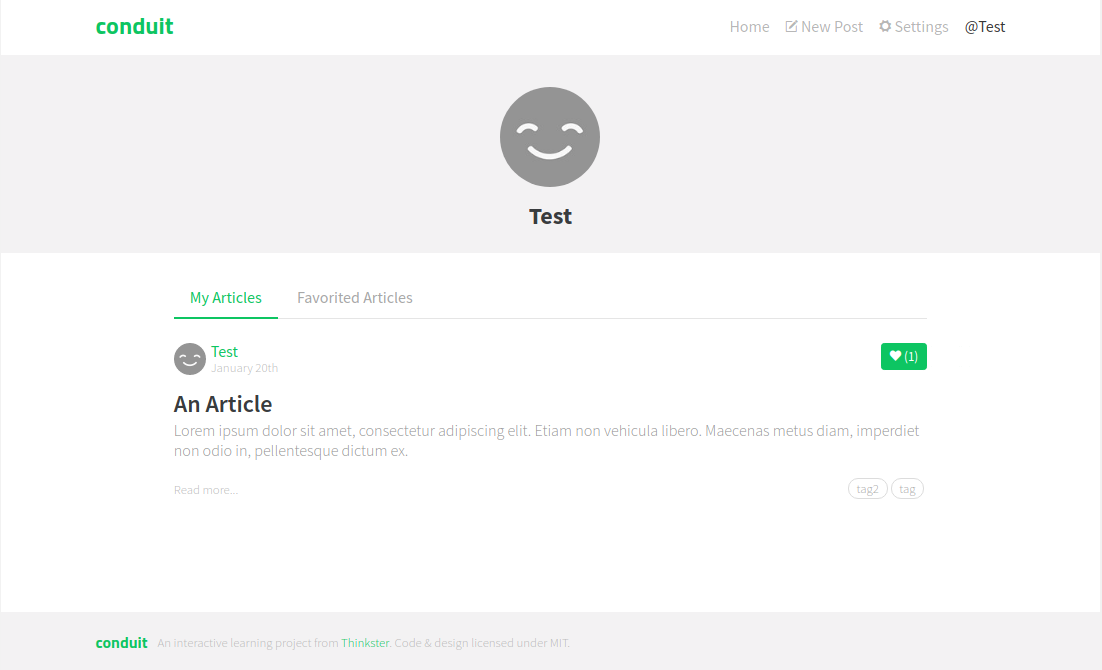
\includegraphics[width=.9\linewidth]{obrazky-figures/screenshot-realworld.png}
\caption{The RealWorld application \label{realworld-app}}
\end{figure}

The created application, illustrated in Figure \ref{realworld-app}, fulfills all
requirements of the specification and of the PWA checklist. As with HNPWA, it
would be possible to improve the application by using a custom server for
prerendering and for unifying the Servant types of the API and the application
into a single large type.

\chapter{Conclusion}
\label{sec:org76fbcfd}
In this work, I have led the reader from a general introduction to modern Web
technologies, through an overview of the capabilities of contemporary Web
frameworks, to an analysis of the capabilities of Haskell on the frontend and
specifically the state of available features in its library ecosystem. In the
second half of this work, I have designed and implemented three components, a
router, a service worker generator with supporting libraries, and a key-value
browser storage library.

\section{Evaluation}
\label{sec:orgd40c3a3}
While these components do not comprise a framework equivalent to the most
popular JavaScript frameworks, they together give developers a set of
functionality that is mostly equivalent to minimalist frameworks in JavaScript,
and they make a significant contribution to the ecosystem of Haskell on the
frontend. They enable creating Progressive Web Applications in Haskell, which
was the set goal of this work, and they also set the groundwork for further work
in this area. I also believe that the analysis done in the first part of this
work is a significant contribution itself, identifying the deficiencies in the
Haskell ecosystem, possibly guiding future projects.

\section{Future work}
\label{sec:org1d95258}
The work that needs to immediately follow the submission of this thesis is
publishing the components created here and seeking feedback from the Haskell
community. This includes fulfilling all the formal requirements necessary for
publishing the individual packages to Hackage, the package repository for
Haskell, and writing up their documentation in two tiers: API documentation and
user manuals. For the manuals and showcases, I will likely reuse some of the
case studies presented in the previous chapter.

I expect to spend some time adapting my work according to any feedback from the
community: expanding documentation, creating adapters to other libraries,
implementing more requested functionality, and other necessary work.

With the libraries implemented in this work, there is, however, still a number of
capabilities that Haskell lacks, compared to developing browser applications in
JavaScript:

\begin{itemize}
\item a palette of pre-built GUI components,
\item internationalization,
\item a unified command-line interface to build tools,
\item code generation, and
\item debugging tools for the frontend, e.g.~variable watching, inspecting application state
\end{itemize}

There is also a number of other ideas with various usefulness that would make
building web applications in Haskell easier. Some are natural extensions of the
implemented components, others are independent projects that implement other
functionality that would make building web applications in Haskell easier. What
follows is an incomplete list of such project topics:

\begin{itemize}
\item CSS-in-Haskell (similar to CSS-in-JS),
\item crash reports (traceback, application state) for the browser,
\item end-to-end tests that can run assertions on both the client and server,
\item dynamic user-provided content, i.e. HTML-like markup that can use preregistered named
components, a user-friendly editor,
\item typed components that use assets, like \texttt{<img>} or \texttt{<link>,}
\item forms: a set of components, validation, automatic derivation from a datatype,
\item a query language for browser storage, using IndexedDB,
\item automatic synchronization for browser storage,
\item authentication in the router: ``user is logged-in'', ``user has role X'', ``user
can perform action Y'',
\item HTTP/2 Push support on the server: sending all necessary assets together with
the first request,
\item WebIDL and a JavaScript-generating DSL for service workers,
\item effect system for Reflex, as a more flexible extension mechanism, and
\item serializable effects that can be interpreted both in the browser or on the
server if the client is missing required data.
\end{itemize}

To summarize this work, I have studied the current state of Haskell on the
frontend, expanded the library ecosystem with three new additions, implemented a
number of example applications, and suggested follow-up projects to remedy the
remaining deficiencies compared to the features available in JavaScript.

% * (bibliography, start of appendix)                           :ignoreheading:
\makeatletter
\def\@openbib@code{\addcontentsline{toc}{chapter}{Bibliography}}
\makeatother
\bibliographystyle{bib-styles/englishiso}

\begin{flushleft}
\bibliography{projekt}
\end{flushleft}
\iftwoside\cleardoublepage\fi

% Appendices
\appendix
\appendixpage
\iftwoside\cleardoublepage\fi

\startcontents[chapters]
% \setlength{\parskip}{0pt}
% \printcontents[chapters]{l}{0}{\setcounter{tocdepth}{2}}
% \setlength{\parskip}{0.5\bigskipamount}
\iftwoside\cleardoublepage\fi

\chapter{Contents of the attached data storage}
\label{sec:orgd5043bb}

\begin{itemize}
\item \texttt{doc-final-thesis/}, the source files for this thesis and its rendered PDF
version,
\item \texttt{doc-midterm-report/}, the source files and rendered PDF version of the midterm
report of this work,
\item \texttt{doc-midterm-presentation/}, the source files and rendered PDF version of the midterm
presentation of this work,
\item \texttt{README.md}, the usage instructions for the following source files,
\item \texttt{src/tapaw-route/}, the routing library created in this work,
\item \texttt{src/tapaw-serviceworker/}, the service worker library created in this work,
\item \texttt{src/tapaw-storage/}, the storage library created in this work,
\item \texttt{src/tapaw-webmanifest/}, the Web App Manifest library created in this work,
\item \texttt{src-demo/tapaw-7guis/}, a simple set of GUI components originally intended as
another demonstration application,
\item \texttt{src-demo/tapaw-todomvc/}, the TodoMVC demonstration application,
\item \texttt{src-demo/tapaw-hnpwa/}, the HNPWA demonstration application,
\item \texttt{src-demo/tapaw-realworld/}, the RealWorld demonstration application,
\item \texttt{src-snippets/}, a set of code snippets written during the process of writing
this thesis, especially:
\begin{itemize}
\item \texttt{deployment-nixops/}, an example of application deployment using NixOps,
\item \texttt{skeleton/}, a minimal project skeleton for a browser application,
\item \texttt{storage-tagged/}, an alternate version of the storage library, and
\item \texttt{editor-emacs/}, a pre-configured instance of the Emacs editor usable for
exploring the packages in this work
\end{itemize}
\end{itemize}
\end{document}